\documentclass[a4paper, 12pt]{article}
\usepackage{graphicx}
\usepackage{float}
\usepackage{listings}
\usepackage[UTF8]{ctex}
\usepackage{xcolor}
\setlength{\parindent}{2em}
\lstdefinestyle{mybash}{
    language=bash,                 % 设置语言为 Bash[reference:8]
    basicstyle=\small\ttfamily,    % 基础字体：使用等宽字体[reference:9][reference:10]
    keywordstyle=\color{blue},     % 关键字颜色[reference:11][reference:12]
    keywordstyle={[2]\color{cyan}},% 第二组关键字颜色[reference:13]
    commentstyle=\itshape\color{orange!70!black}, % 注释样式：斜体 + 橙色[reference:14]
    stringstyle=\color{teal},      % 字符串颜色[reference:15]
    backgroundcolor=\color{yellow!10}, % 背景色：浅黄色[reference:16][reference:17]
    frame=single,                  % 代码框样式[reference:18]
    numbers=left,                  % 在左侧显示行号[reference:19]
    numberstyle=\tiny\color{gray}, % 行号样式[reference:20]
    breaklines=true,               % 自动换行
    showstringspaces=false,        % 不显示字符串中的空格[reference:21][reference:22]
}
\begin{document}
  \title{Week04 实验报告}
  \author{mrw1114}
  \date{September, 14th}
  \maketitle
  \section{个人信息}
  \begin{itemize}
    \item 姓名：王俊杰
    \item 学号：25020007122
    \item Github 仓库链接：https://github.com/mrw1114/fundamentals-of-system-dev-tools
  \end{itemize}
  \section{课上实验}
    \subsection{第13题：建立可执行的本地质量门禁}
      \subsubsection{复制项目并修改配置文件}
      在 q10 目录的上级执行 cp -r ./q10 q13 复制项目。随后进入 q13 目录，修改 pyproject.toml 文件，加入 ruff 和 pytest 的最小配置，配置了 line-length（单行最大字符数，默认88）、target-version（项目版本） 以及 testpaths（pytest 寻找测试文件的默认路径）。
      \noindent
      \begin{figure}[H]
        \centering
        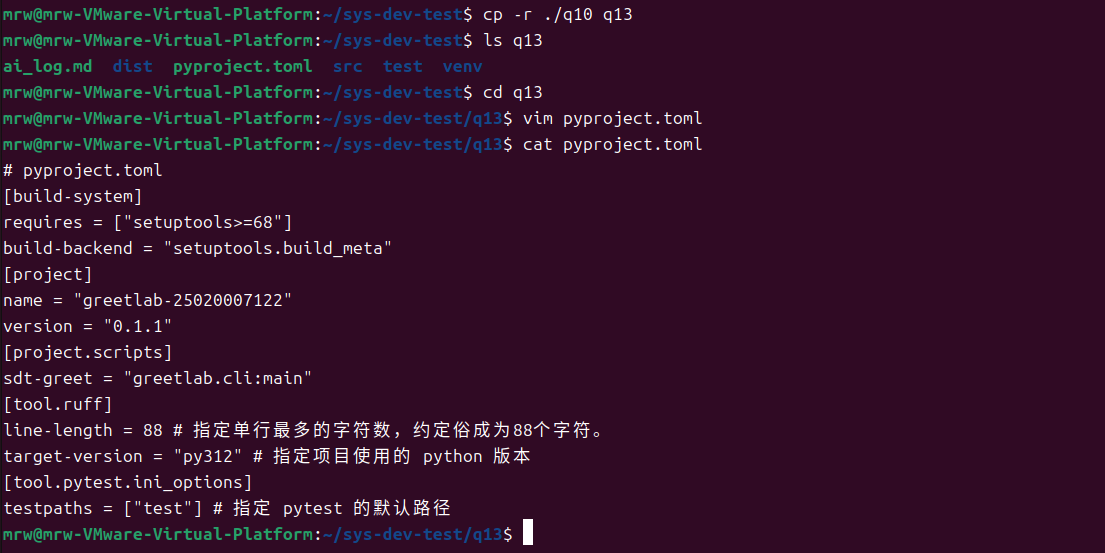
\includegraphics[width=\textwidth]{13-1.png}
        \caption{在 pyproject.toml 中添加 ruff 和 pytest 的最小配置}
        \label{13-1}
      \end{figure}
      \subsubsection{补充测试用例}
      新建 test/test\_cli.py 文件，补充正常姓名和空白姓名测试，正常姓名测试中 stdout 应有"Hello, 王俊杰"，空白姓名测试返回码应为2。
      \noindent
      \begin{figure}[H]
        \centering
        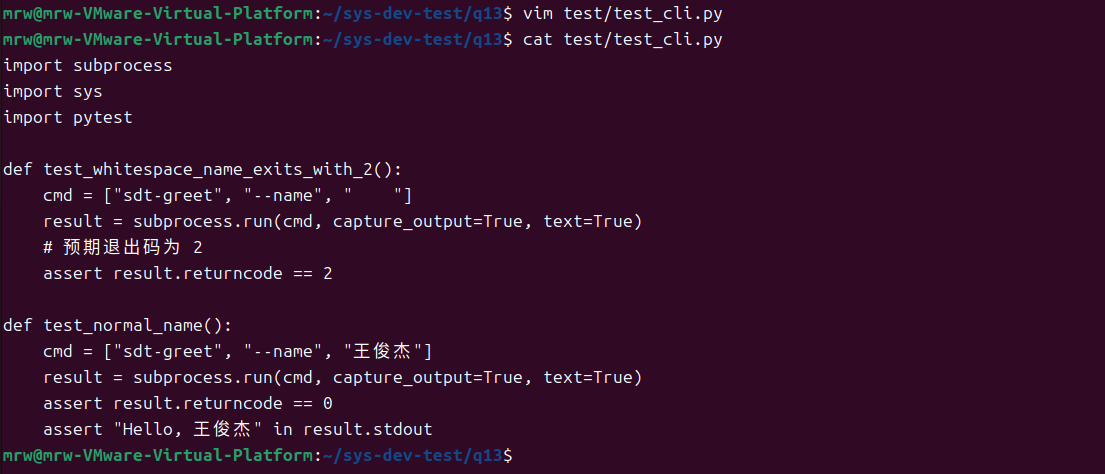
\includegraphics[width=\textwidth]{13-2.png}
        \caption{test\_cli.py 中的测试内容}
        \label{13-2}
      \end{figure}
      \subsubsection{运行质量检查并修复问题}
      执行 ruff format 和 ruff check，发现 EXE002（缺少 shebang）、I001（导入未排序）、F401（未使用导入）、PLW1510（subprocess.run 缺少 check 参数）等错误。运行 pytest 时，test\_normal\_name 测试失败。随后执行 ruff check --fix 自动修复部分问题，但 EXE002 和 PLW1510 无法自动修复：EXE002 需要手动移除文件可执行权限或添加 shebang；PLW1510 需要人工判断 subprocess.run 的 check 参数应设为 True 还是 False （设置为 True 时，subprocess.run 若有非0返回码则抛出异常）。手动修改 test/test\_cli.py，添加 check=False 参数；随后鉴于包文件和测试文件无需直接执行，使用 chmod -x 移除源文件和测试文件的可执行权限。再次运行 ruff check，显示全部通过。最后编写 check.sh 脚本，依次执行 ruff format --check、ruff check 和 pytest，使用 set -e 确保出错时立即退出，并赋予执行权限。
      \noindent
      \begin{figure}[H]
        \centering
        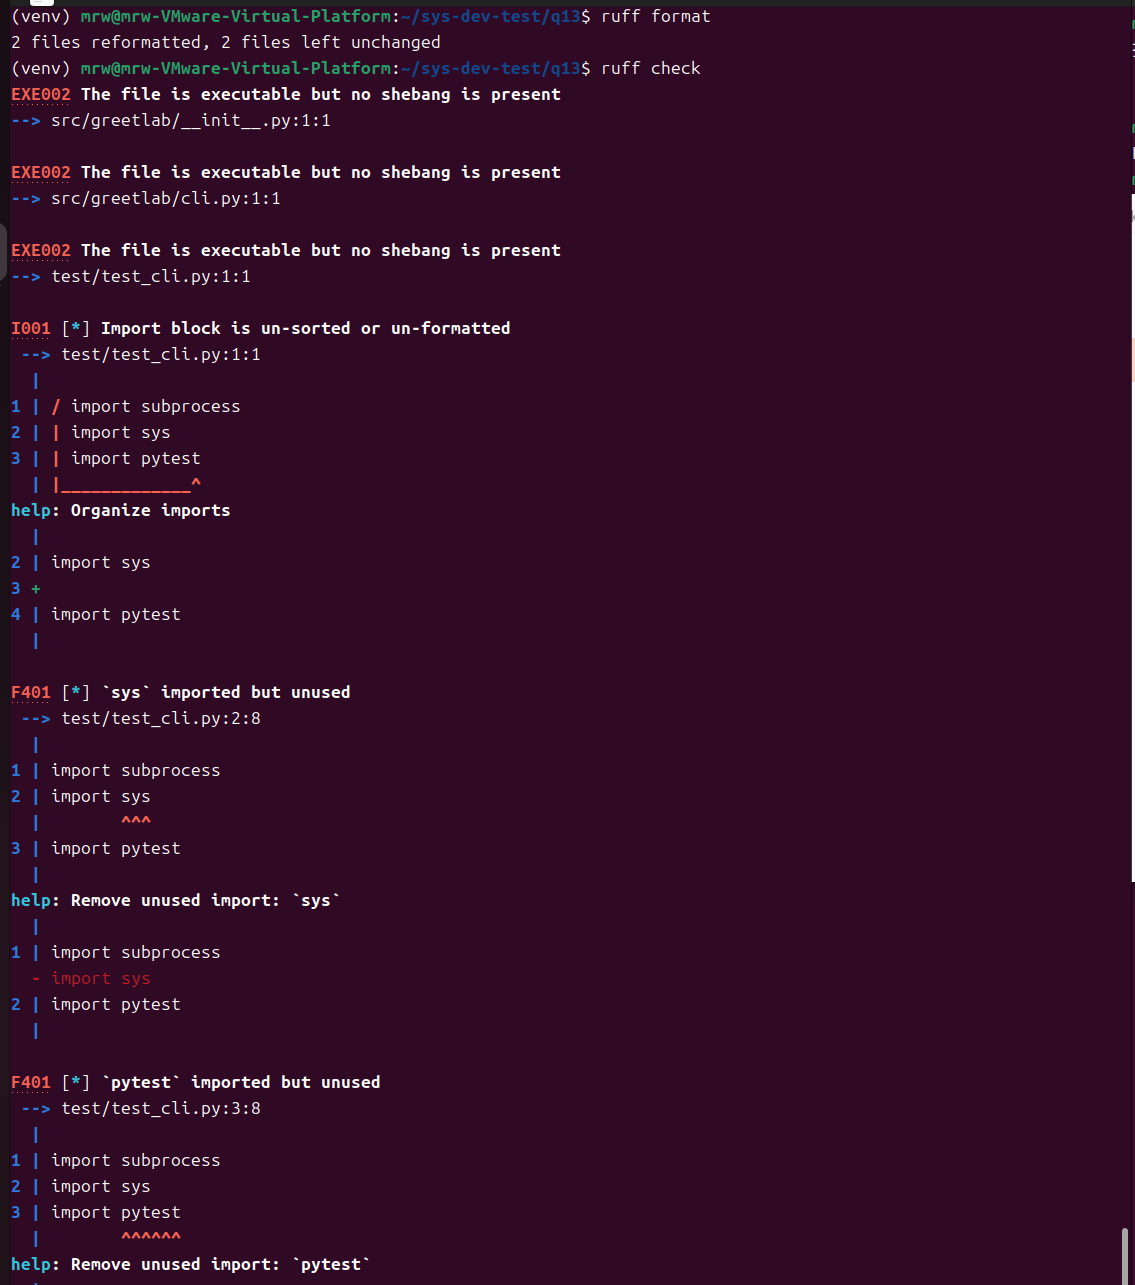
\includegraphics[width=\textwidth]{13-3-1.png}
        \caption{运行 ruff format 和 ruff check 的前半段输出}
        \label{13-3-1}
      \end{figure}
      \noindent
      \begin{figure}[H]
        \centering
        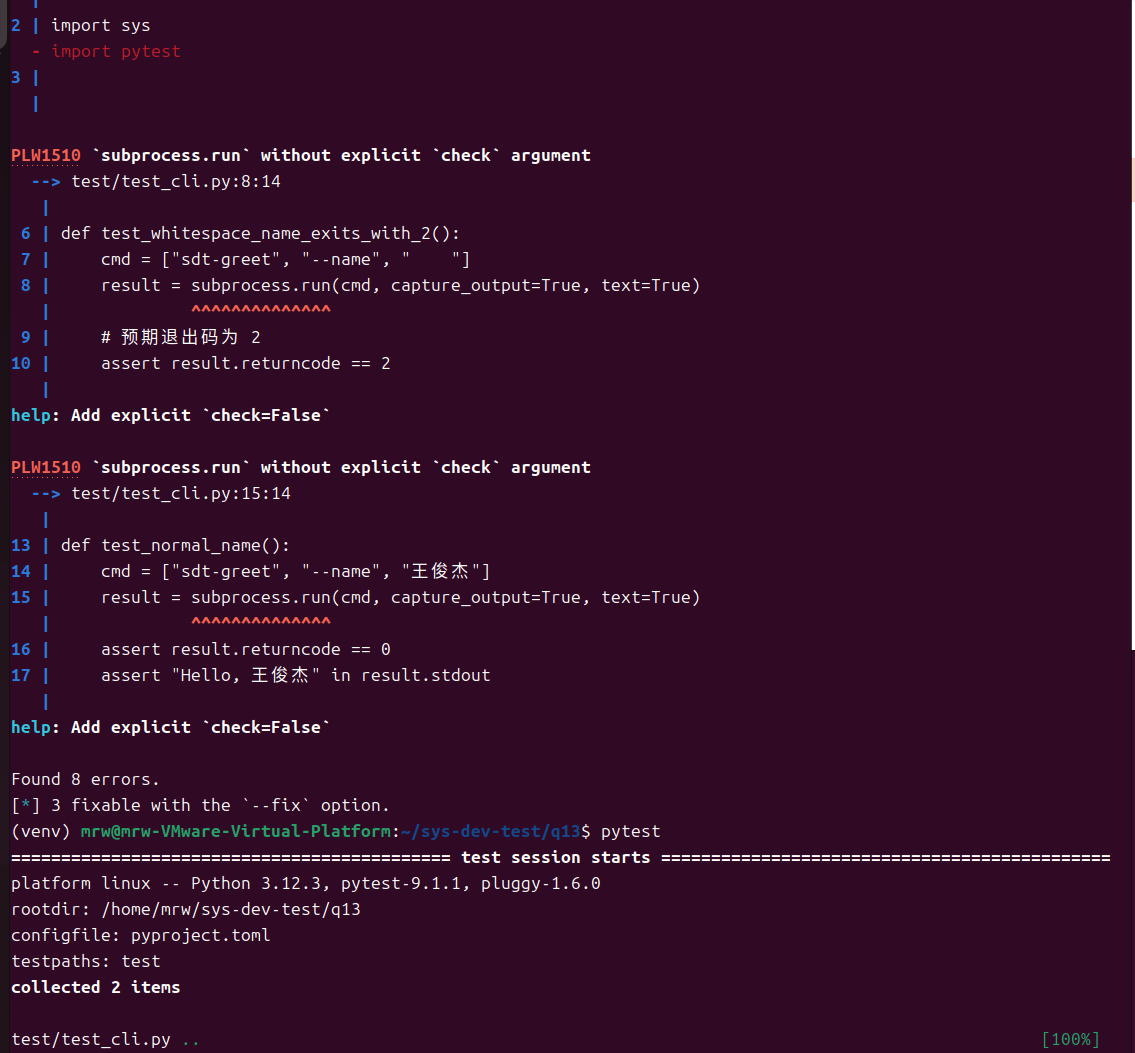
\includegraphics[width=\textwidth]{13-3-2.png}
        \caption{ruff check 的后半段输出与 pytest 失败结果}
        \label{13-3-2}
      \end{figure}
      \noindent
      \begin{figure}[H]
        \centering
        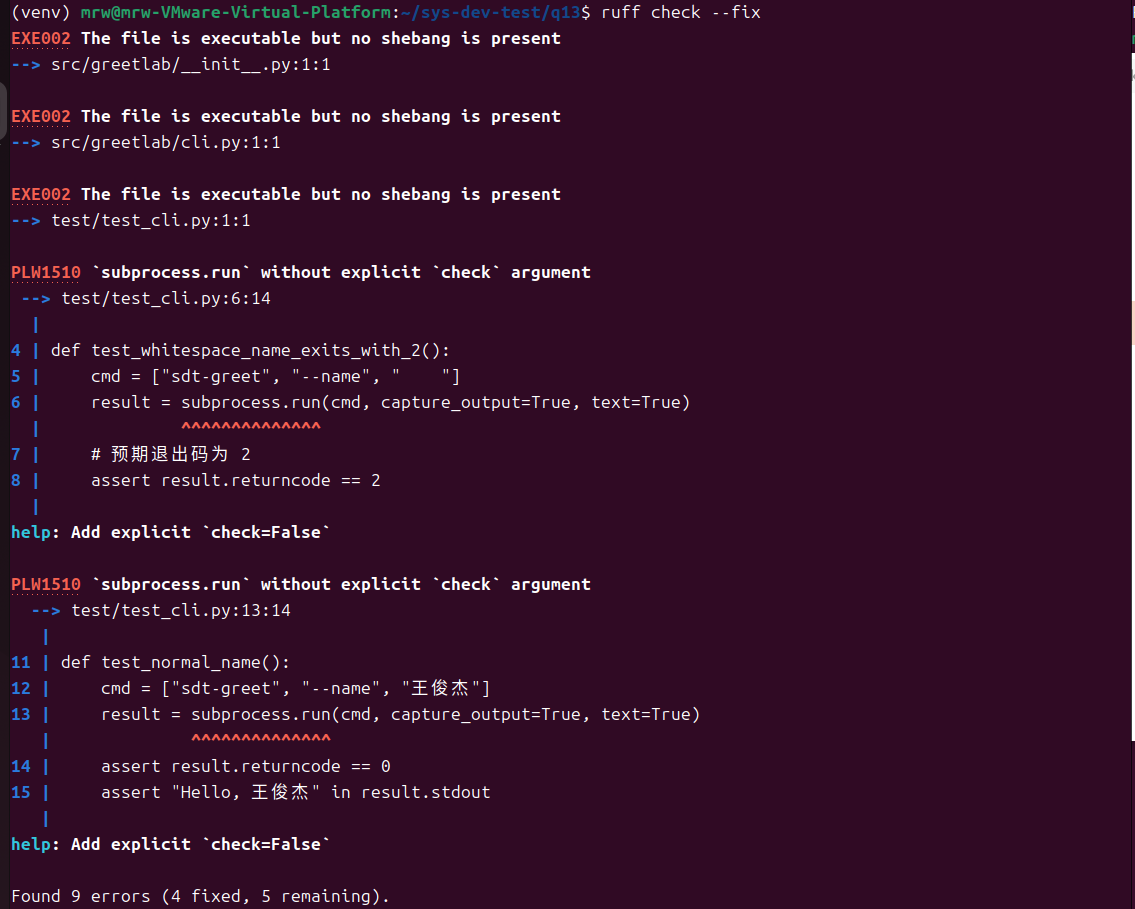
\includegraphics[width=\textwidth]{13-3-3.png}
        \caption{使用 ruff check --fix 自动修复后剩余的无法自动修复的问题}
        \label{13-3-3}
      \end{figure}
      \noindent
      \begin{figure}[H]
        \centering
        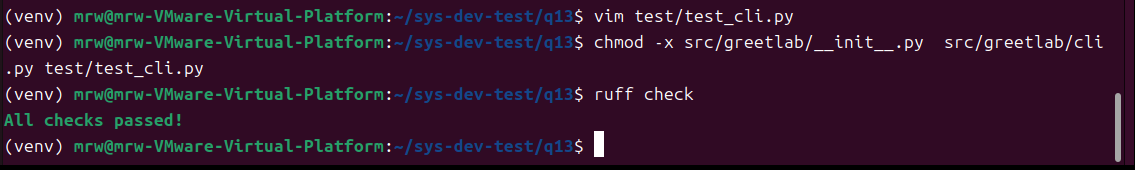
\includegraphics[width=\textwidth]{13-3-4.png}
        \caption{修复剩余问题后 ruff check 通过}
        \label{13-3-4}
      \end{figure}
      \subsubsection{运行 check.sh 验证}
      编写并执行 ./check.sh，所有检查通过并成功返回 0。
      \noindent
      \begin{figure}[H]
        \centering
        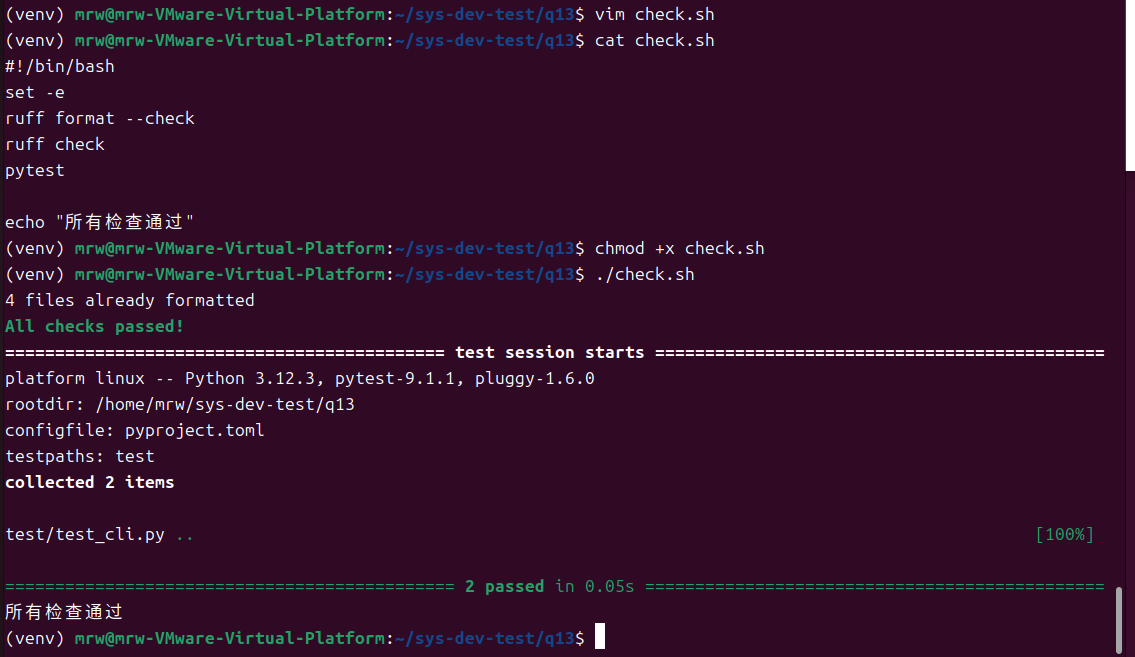
\includegraphics[width=\textwidth]{13-4.png}
        \caption{check.sh 的编写与执行成功}
        \label{13-4}
      \end{figure}

    \subsection{第14题：让Make只重建真正受影响的产物}
      \subsubsection{创建源文件}
      在 q14 目录下创建给定的 data.csv、stats.py、build\_report.py 和 report.md 文件。
      \noindent
      \begin{figure}[H]
        \centering
        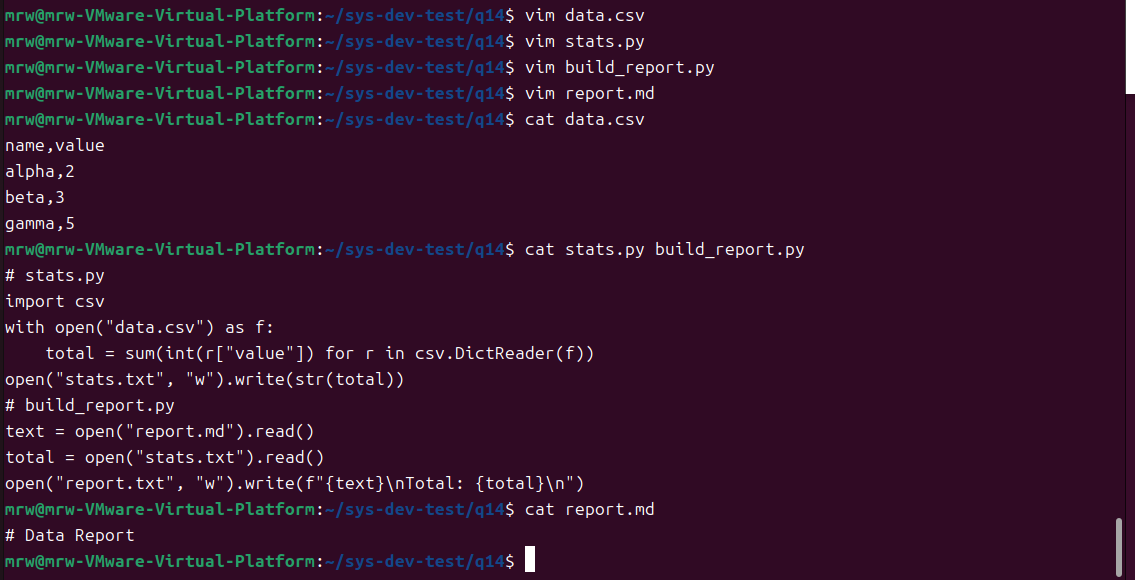
\includegraphics[width=\textwidth]{14-1.png}
        \caption{创建给定的源文件}
        \label{14-1}
      \end{figure}
      \subsubsection{编写Makefile}
      编写 Makefile，包含 all、stats.txt、report.txt 和 clean 目标，列出数据文件、脚本和中间产物的依赖关系。其中 .PHONY 声明表示将对应目标设置为伪目标，因为 make 优先将目标视为对应的文件，而 all 表示构建系统默认的目标，其依赖表示构建系统默认构建的产物；clean 无依赖也不生成产物，其动作用于清除构建过程中的中间产物。如果不进行 .PHONY 声明，则当待构建的目录中存在名称为 all 或 clean 的文件时，可能无法正确执行 make 和 make clean 等命令。
      \noindent
      \begin{figure}[H]
        \centering
        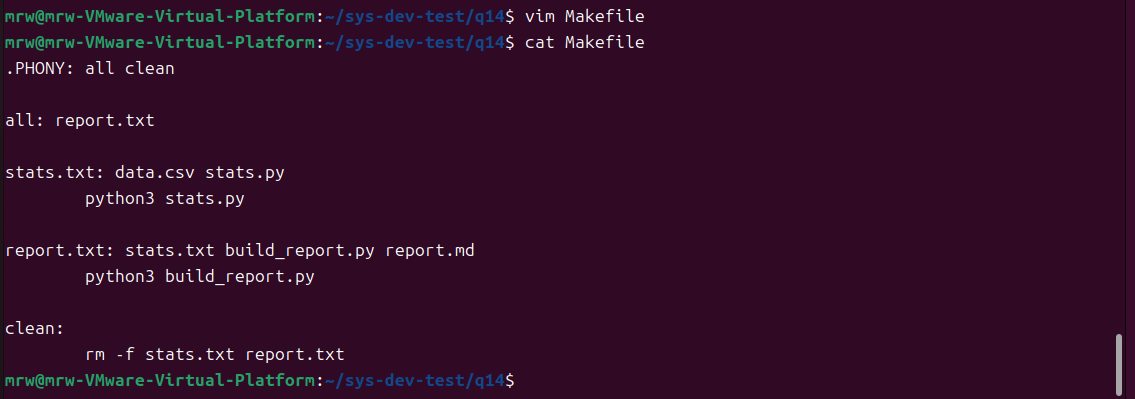
\includegraphics[width=\textwidth]{14-2.png}
        \caption{Makefile 内容}
        \label{14-2}
      \end{figure}
      \subsubsection{验证构建逻辑}
      首次执行 make，成功生成 stats.txt 和 report.txt。第二次执行 make，未执行配方更新产物。执行 touch data.csv 后再次 make，发现 stats.txt 和 report.txt 重新生成。执行 make clean，仅删除生成物而源文件不受影响。
      \noindent
      \begin{figure}[H]
        \centering
        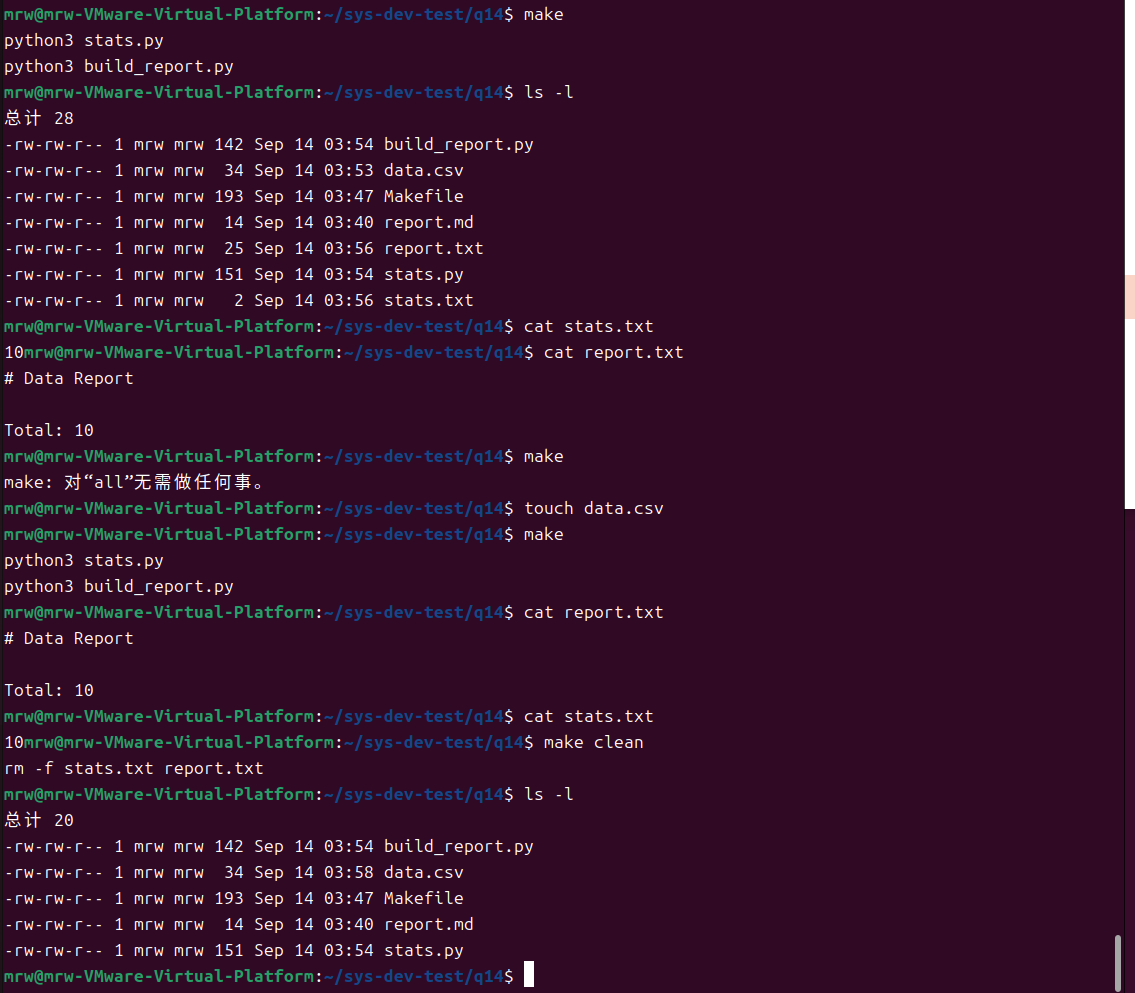
\includegraphics[width=\textwidth]{14-3.png}
        \caption{make 产物验证与更新后的 make clean}
        \label{14-3}
      \end{figure}

    \subsection{第15题：把本地API数据转换为可读报告}
      \subsubsection{创建JSON数据并启动本地服务}
      创建 packages.json 文件并填入给定的 JSON 数据。在 q15 目录下运行 python3 -m http.server 8000 启动本地 HTTP 服务。
      \noindent
      \begin{figure}[H]
        \centering
        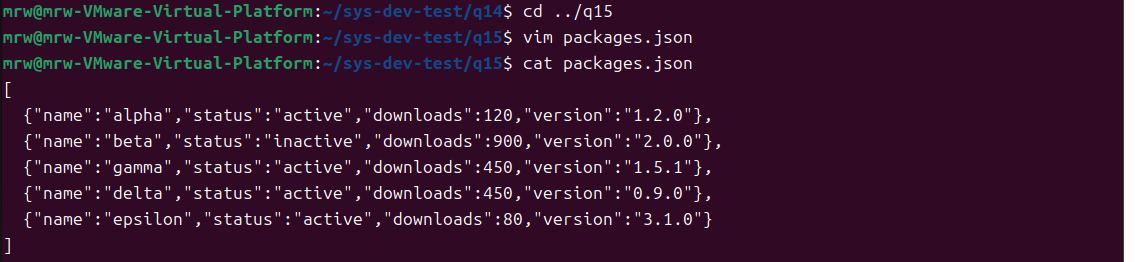
\includegraphics[width=\textwidth]{15-1.png}
        \caption{创建 packages.json 文件}
        \label{15-1}
      \end{figure}
      \subsubsection{编写api\_report.sh生成报告}
      编写 api\_report.sh，使用 curl -fsS 获取 JSON 数据，通过 jq 筛选 status 为 active 且 downloads 不少于 100 的记录，并使用 sort 按 downloads 降序、name 升序排列。最后通过 awk 格式化为 Markdown 表格，写入 summary.md。执行脚本并查看生成的报告。
      \noindent
      \begin{figure}[H]
        \centering
        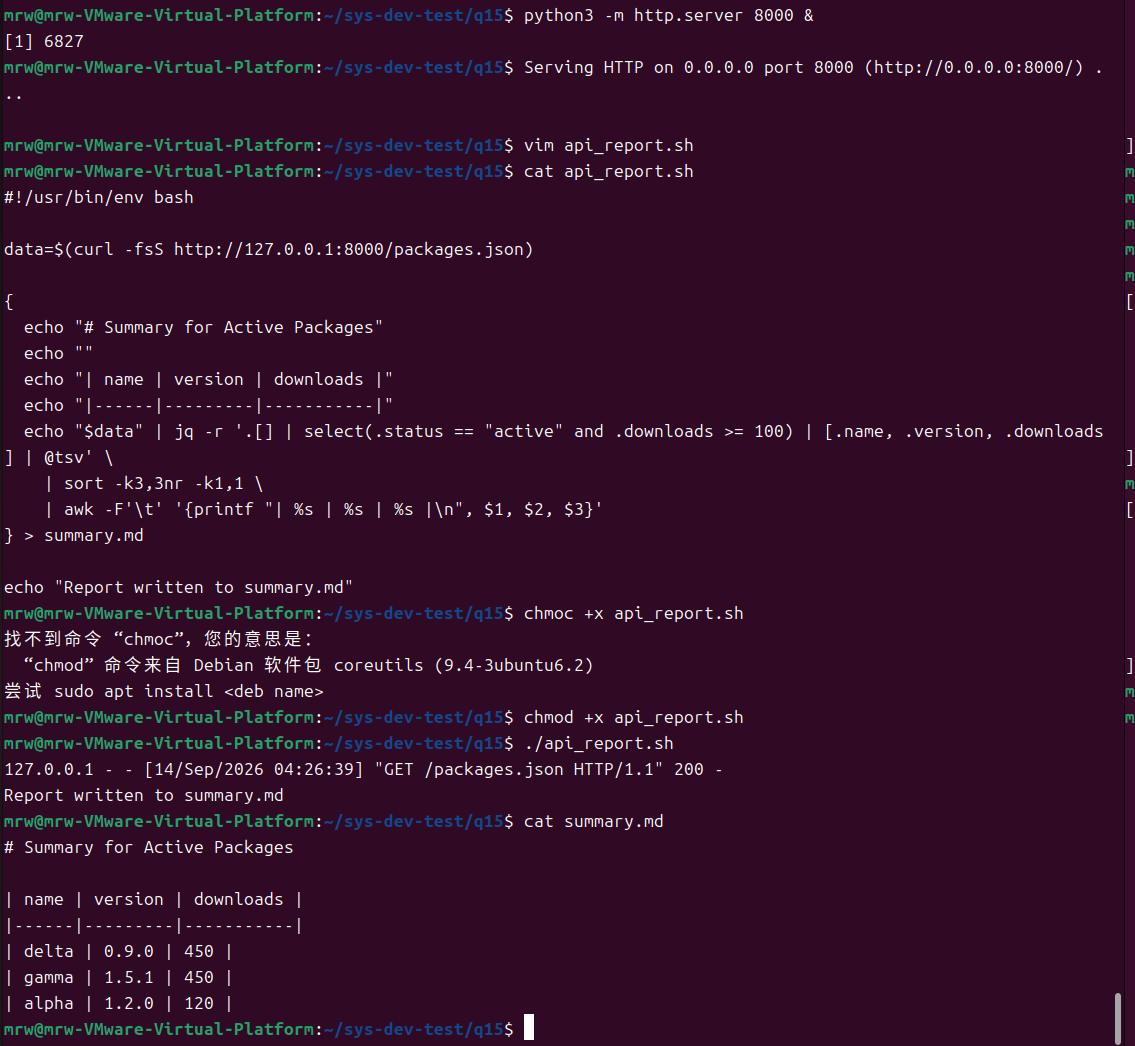
\includegraphics[width=\textwidth]{15-2.png}
        \caption{创建服务器并通过 API 获取信息生成 summary.md}
        \label{15-2}
      \end{figure}

    \subsection{第16题：修复并交付一个陌生的小型工具仓库}
    \noindent
    由于在之前第10题，第13题中没有为 cli.py 添加保护块，导致 pytest 测试只能对 build 并安装的 whl 包进行测试，所以此处 make check 中包含了构建产物，强制重新安装产物，执行 check.sh ，卸载包并删除 build 产物的流程。
      \subsubsection{复制项目并初始化Git}
      执行 cp -r ./q13 q16 复制项目，进入 q16 目录后执行 git init 初始化仓库，并完成初始提交。
      \noindent
      \begin{figure}[H]
        \centering
        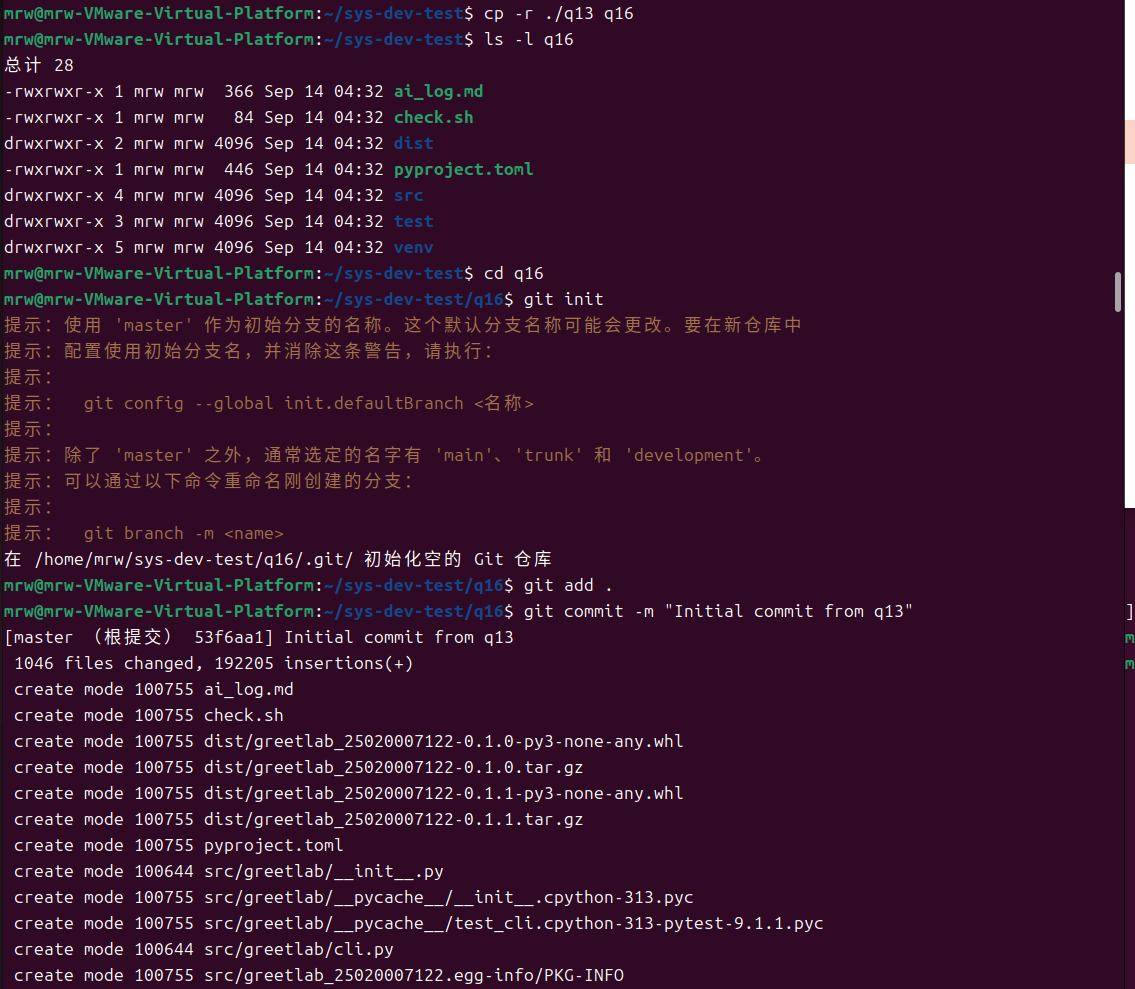
\includegraphics[width=\textwidth]{16-1.png}
        \caption{目录复制与仓库初始化}
        \label{16-1}
      \end{figure}
      \subsubsection{手动制造错误并复现测试失败}
      临时修改 src/greetlab/cli.py，将问候语改为始终返回字面量 "Hello, name!"。执行 check.sh，确认测试失败。随后查看错误实现并改正为正确的 f-string 格式。
      \noindent
      \begin{figure}[H]
        \centering
        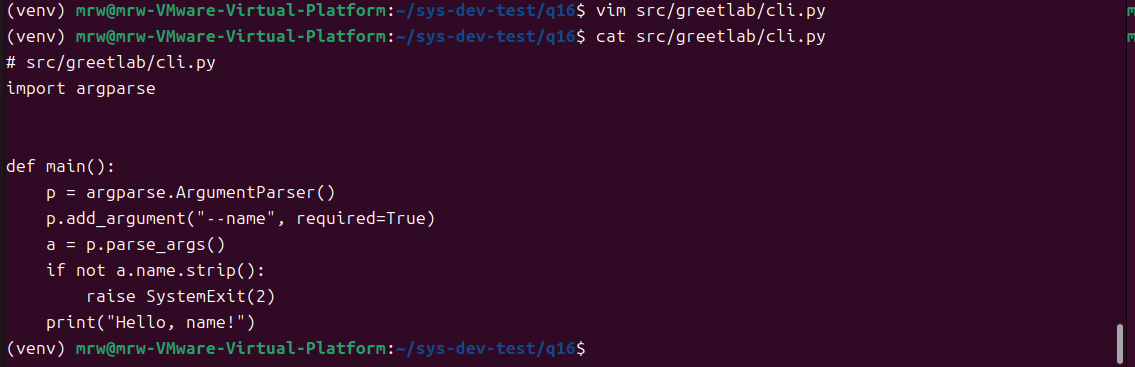
\includegraphics[width=\textwidth]{16-2-1.png}
        \caption{手动制造错误}
        \label{16-2-1}
      \end{figure}
      \noindent
      \begin{figure}[H]
        \centering
        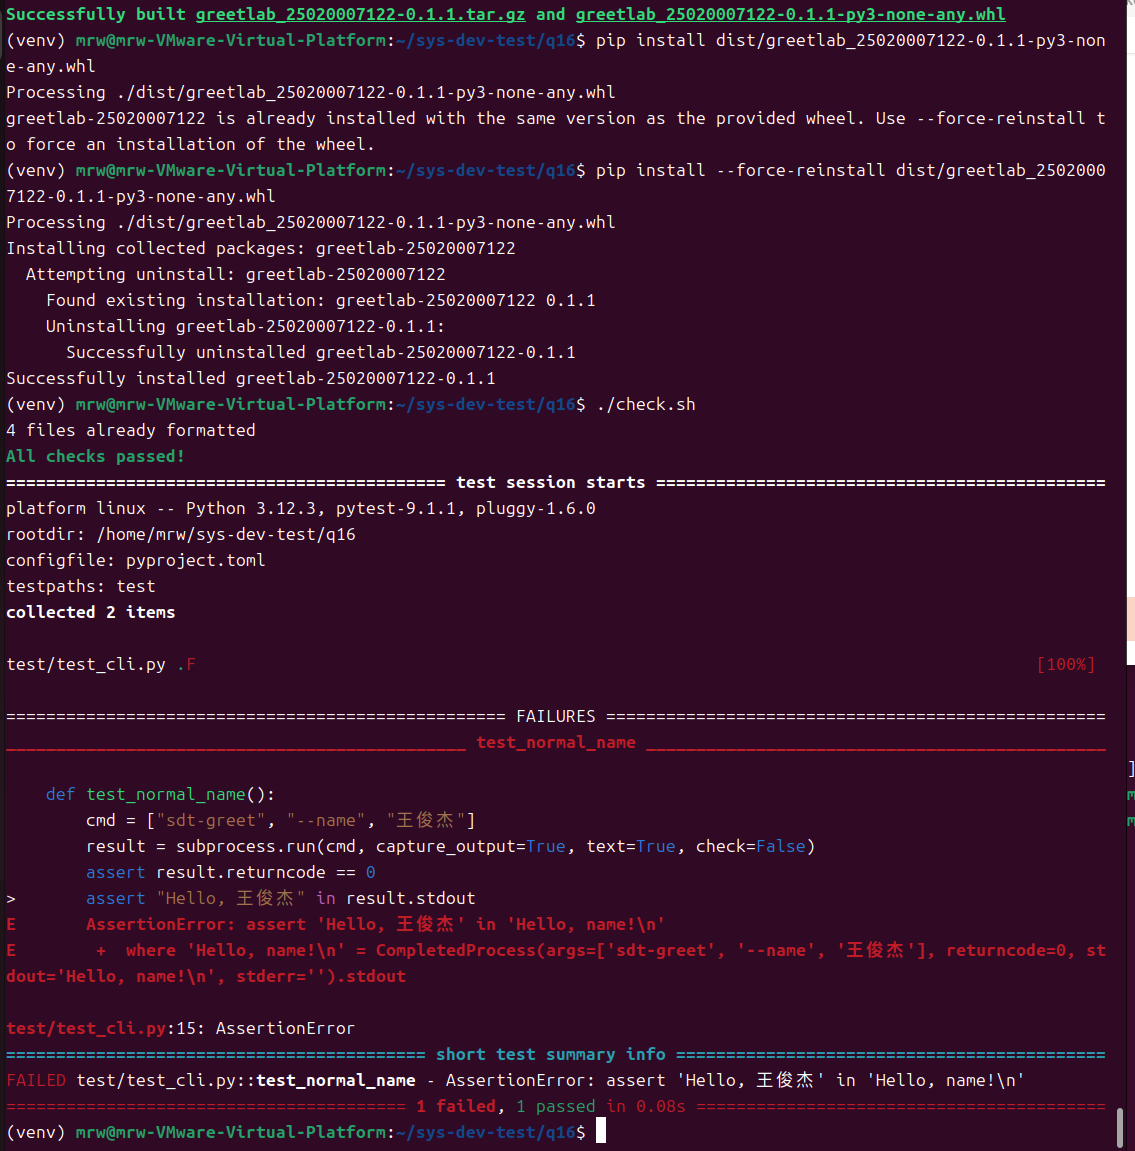
\includegraphics[width=\textwidth]{16-2-2.png}
        \caption{执行 check.sh 的结果（测试失败）}
        \label{16-2-2}
      \end{figure}
      \noindent
      \begin{figure}[H]
        \centering
        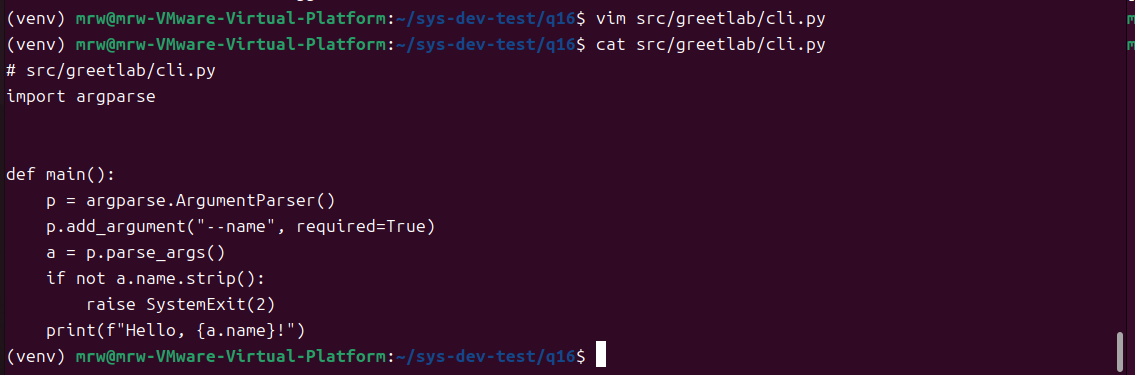
\includegraphics[width=\textwidth]{16-2-3.png}
        \caption{改正错误}
        \label{16-2-3}
      \end{figure}
      \subsubsection{编写Makefile}
      编写包含 check、build 和 clean 的最小 Makefile，其中 check 调用 check.sh，build 生成 wheel。
      \noindent
      \begin{figure}[H]
        \centering
        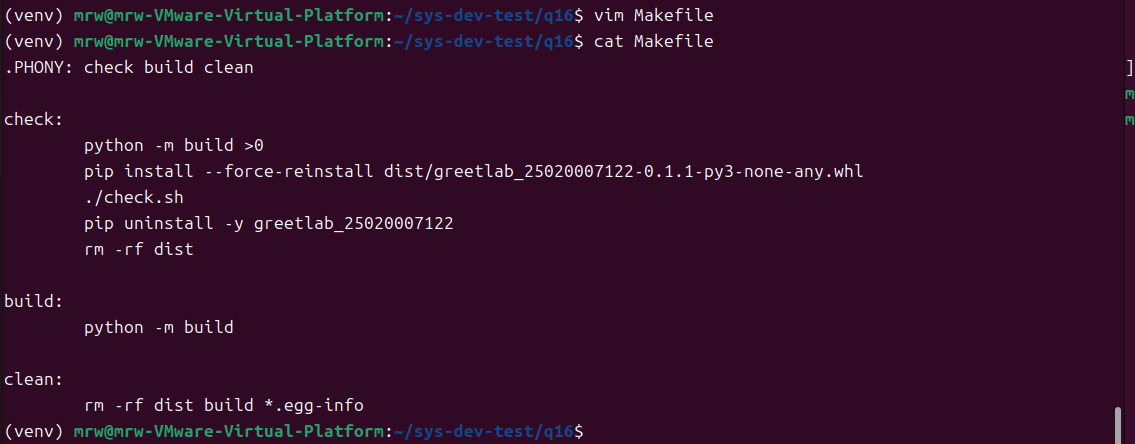
\includegraphics[width=\textwidth]{16-3.png}
        \caption{编写 Makefile}
        \label{16-3}
      \end{figure}
      \subsubsection{运行 make check 和 make build}
      执行 make check 和 make build，验证检查通过并成功构建 wheel。
      \noindent
      \begin{figure}[H]
        \centering
        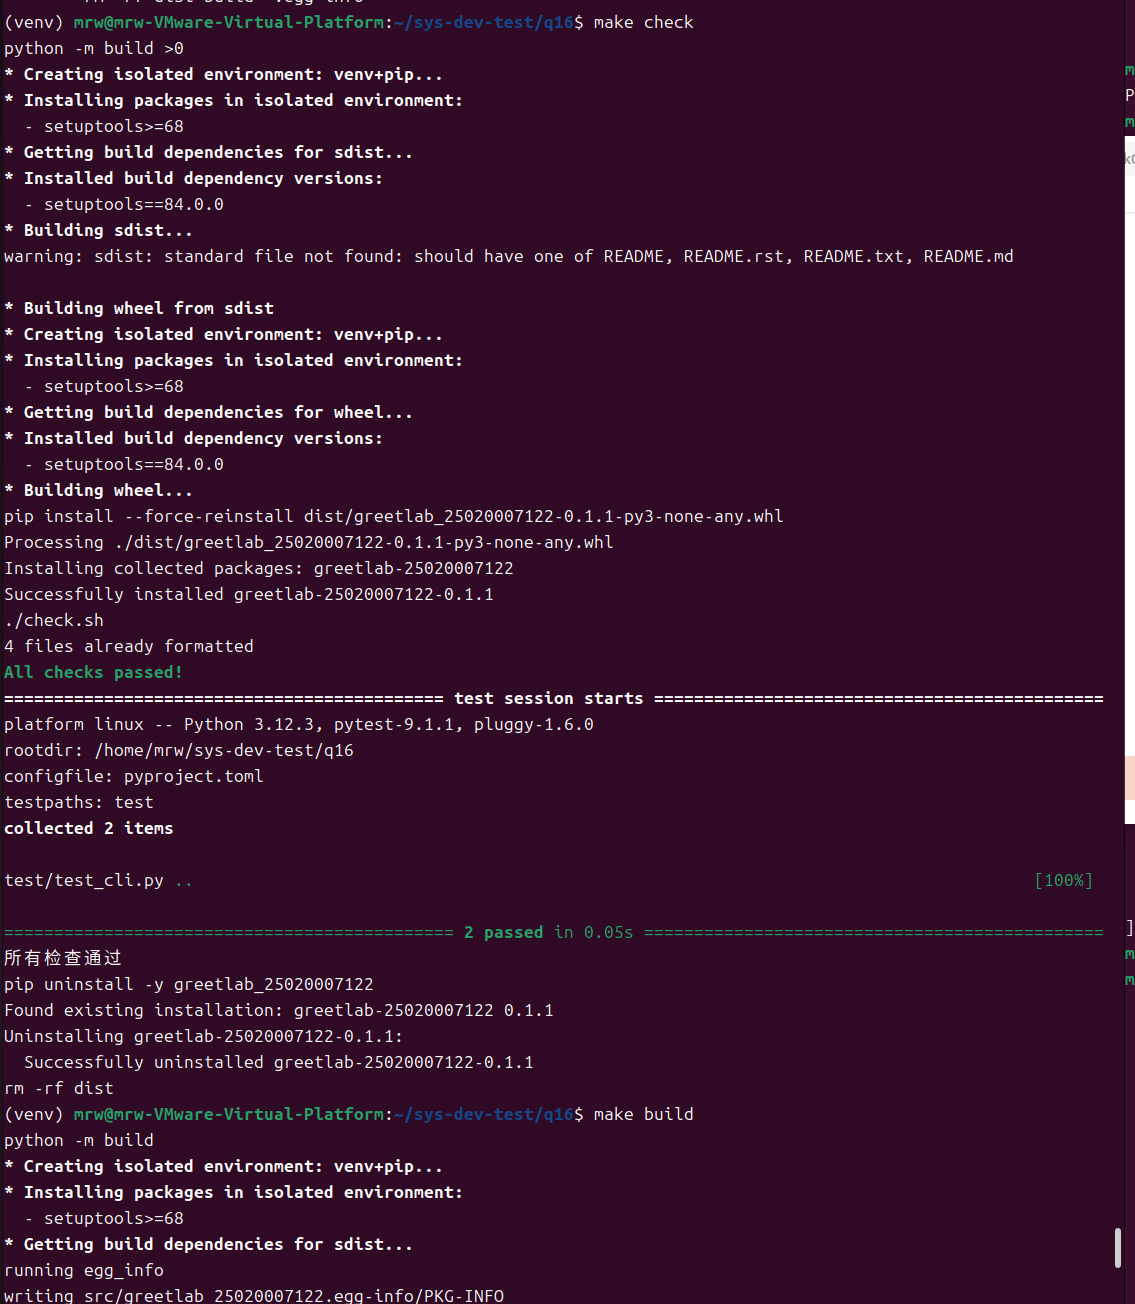
\includegraphics[width=\textwidth]{16-4.png}
        \caption{用 make 进行 check 和 build}
        \label{16-4}
      \end{figure}
      \subsubsection{计算哈希并提交}
      使用 sha256sum 计算 wheel 的 SHA-256 值，编辑 .gitignore 忽略生成物，最后将改动提交为内容聚焦的 Git 提交。
      \noindent
      \begin{figure}[H]
        \centering
        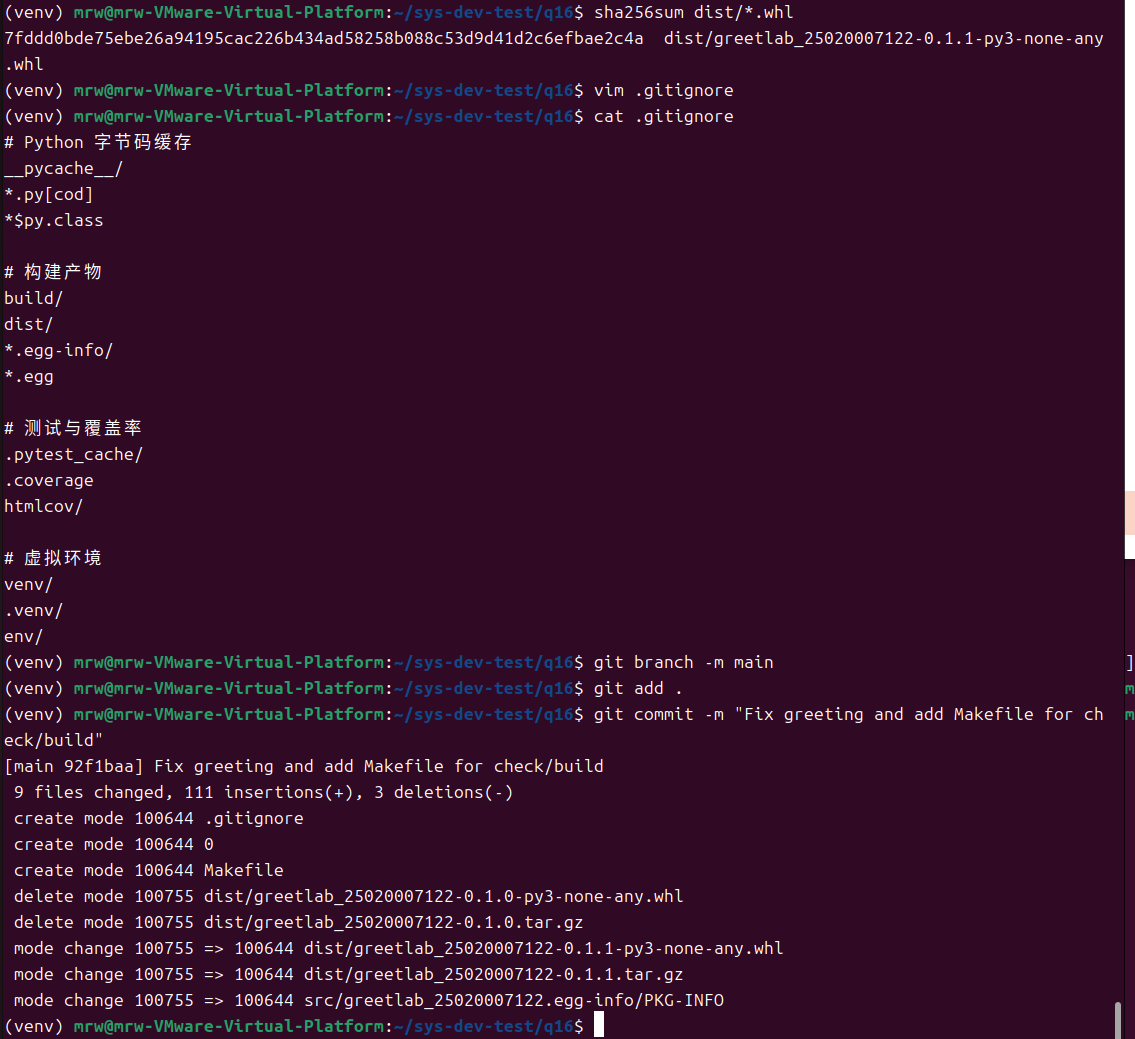
\includegraphics[width=\textwidth]{16-5.png}
        \caption{计算构建产物的 SHA-256、编辑 .gitignore 并提交}
        \label{16-5}
      \end{figure}  
\section{课后练习}
    \subsection{第01题}
      \subsubsection{题目描述}
      试着写一个正则表达式，并使用 grep 命令行工具 在你的代码中查找 subprocess.Popen(..., shell=True) 的出现位置。然后，试着“破坏”这个 regex 模式。semgrep 是否仍然能成功匹配到那些会让你的 grep 调用失效的危险代码？
      \subsubsection{解题步骤}
      在 01 目录下新建 test.py 并写入 subprocess.Popen('echo test', shell=True)，用 \detokenize{grep -rn "subprocess\.Popen\(.*shell=True\)" .} 可以匹配到该调用所在的第 2 行。随后改写 test.py：把 subprocess.Popen 赋给变量 a、把 True 赋给变量 b，再以 \detokenize{a('echo test', shell=b)} 的形式调用。程序仍能执行并输出 test，但同样的 grep 命令无输出，说明 grep 只做文本模式匹配，通过使用赋值等方式改写程序结构可以绕过检测。改用 semgrep 的 python.lang.security.audit.subprocess-shell-true 规则时提示该规则路径不存在，于是改用 \detokenize{semgrep --config=auto .} 从 registry 加载规则扫描；semgrep 基于抽象语法树分析语义，因此仍能匹配到这类被改写后的危险调用。
      \noindent
      \begin{figure}[H]
        \centering
        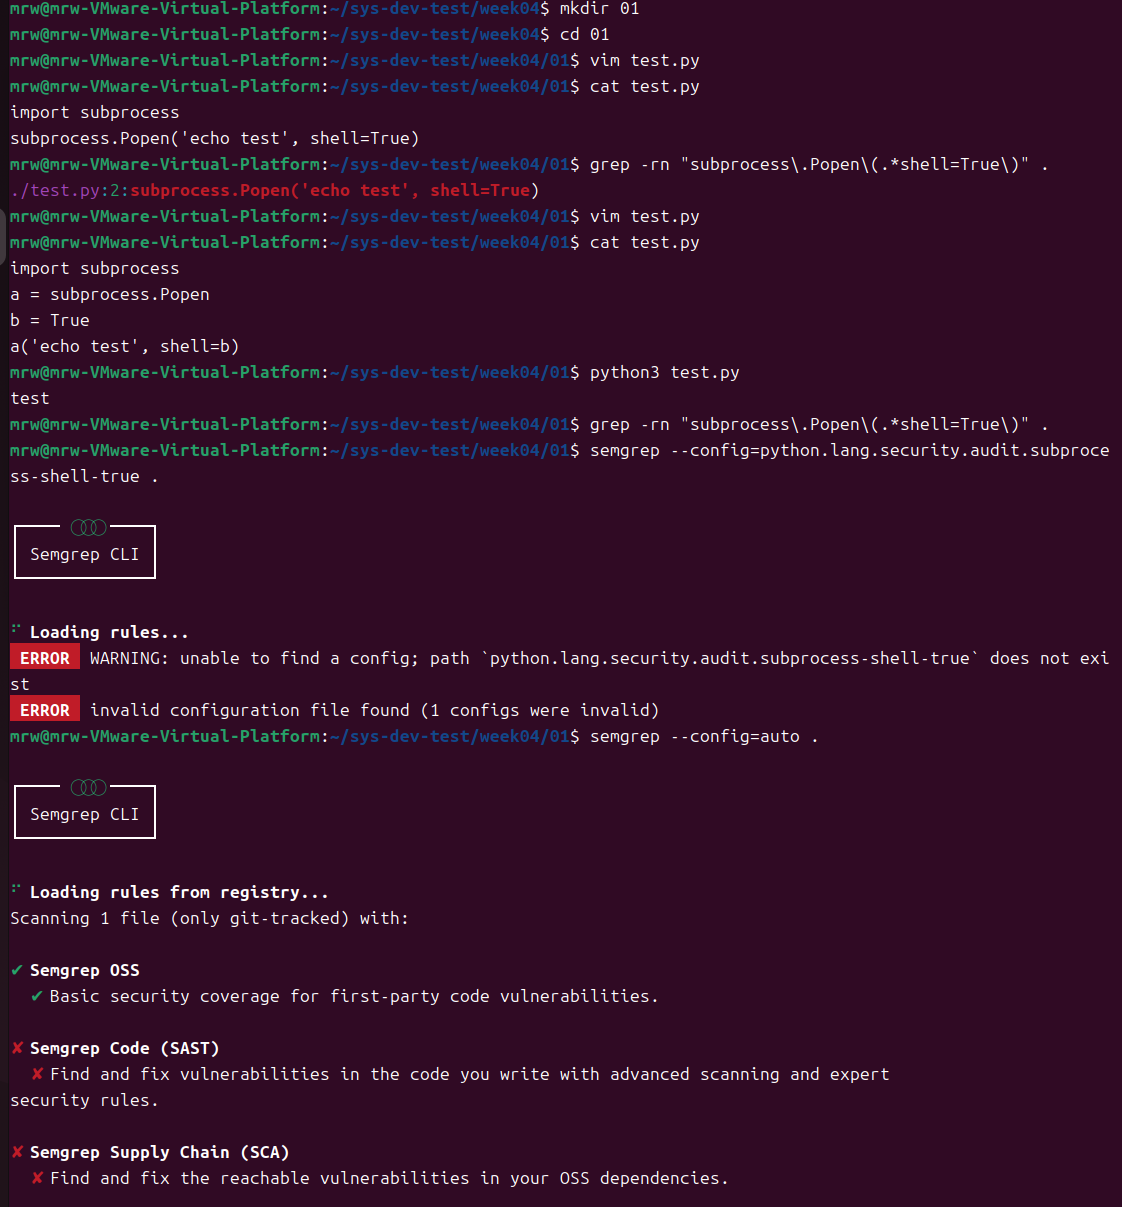
\includegraphics[width=\textwidth]{work04-1.png}
        \caption{grep 匹配危险调用及其被绕过，semgrep 的语义扫描}
        \label{work04-1}
      \end{figure}
    \subsection{第02题}
      \subsubsection{题目描述}
      在你的 IDE 或文本编辑器里练习 regex 查找替换，把这些讲义(https://raw.githubusercontent.com/missing-semester/missing-semester/refs/heads/master/\_2026/code-quality.md) 中的 - Markdown 项目符号标记替换为 * 项目符号标记。注意，直接替换文件中所有的 - 字符是不正确的，因为该字符在文件中还有很多并非项目符号标记的用途。
      \subsubsection{解题步骤}
      在 02 目录下用 curl 下载讲义 code-quality.md，再在 vim 中使用正则替换 :\%s/\^{}-\textbackslash s*/* /，把行首的 - 项目符号替换为 *，共完成 28 处替换。由于 - 在文中还充当减号与分隔线，直接替换所有 - 会误改正文，故使用 \^{} 匹配行首进行避免。
      \noindent
      \begin{figure}[H]
        \centering
        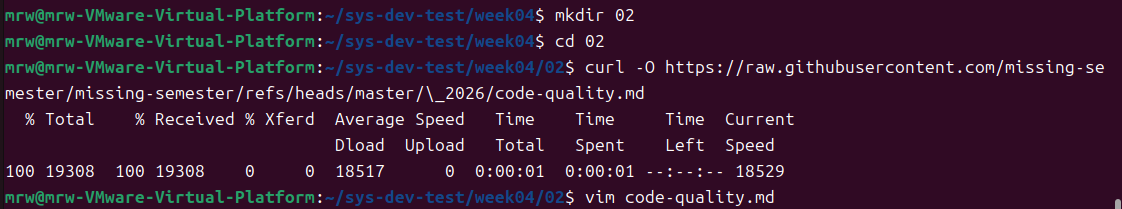
\includegraphics[width=\textwidth]{work04-2-1.png}
        \caption{下载 code-quality.md 并进入 vim 编辑}
        \label{work04-2-1}
      \end{figure}
      \noindent
      \begin{figure}[H]
        \centering
        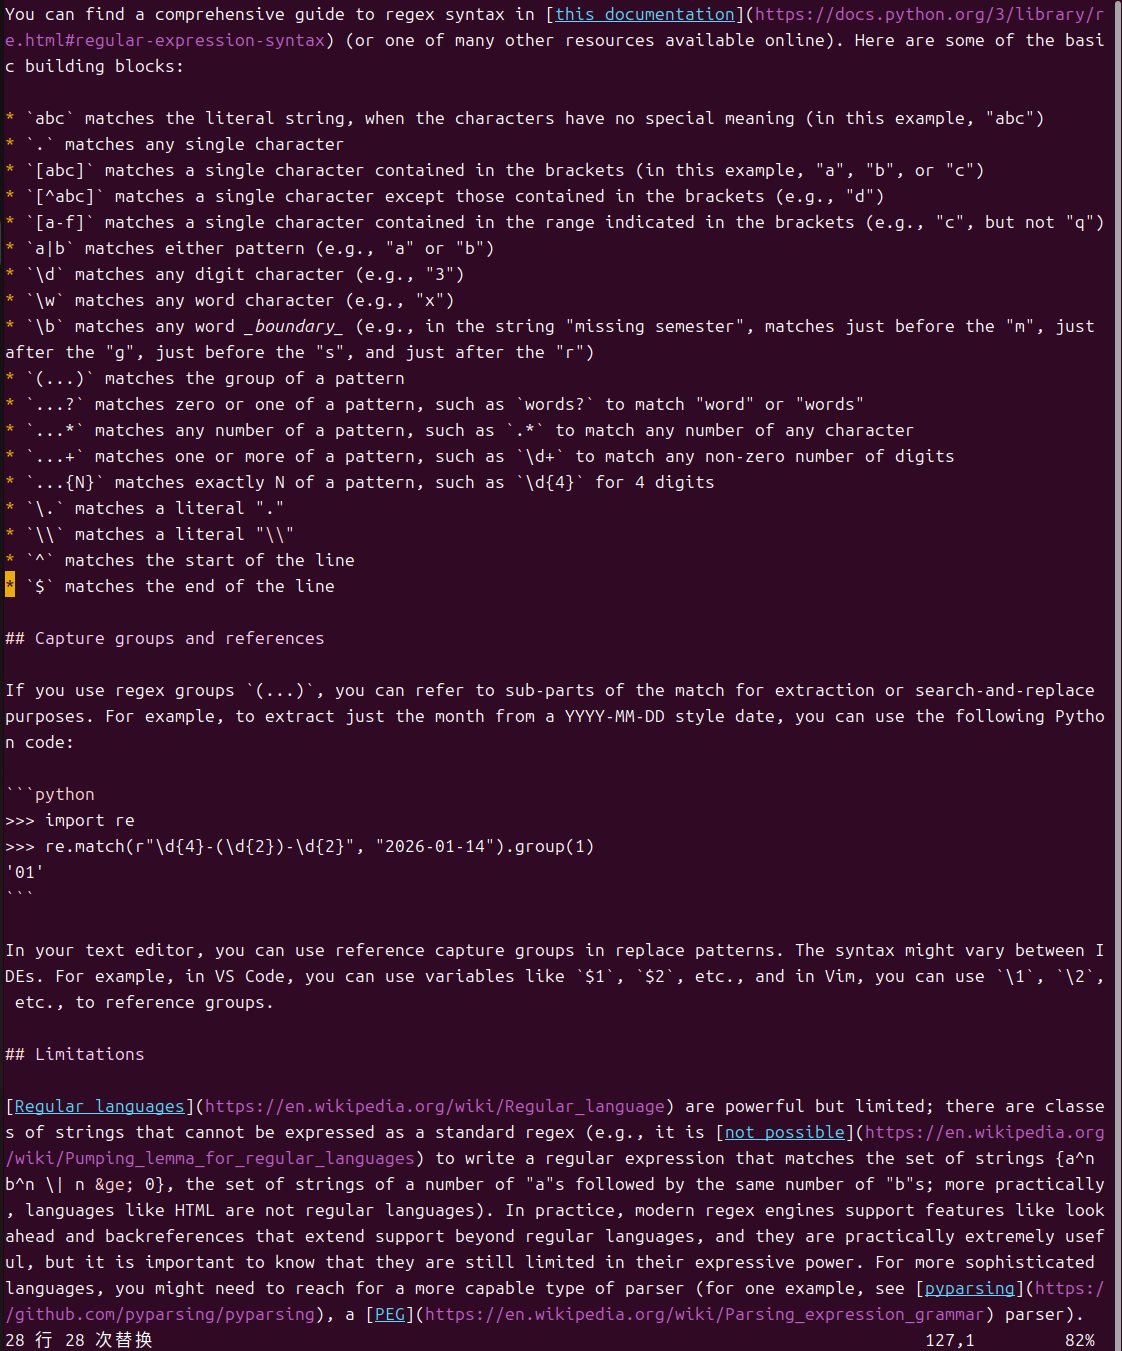
\includegraphics[width=\textwidth]{work04-2-2.png}
        \caption{替换后的 Markdown 文件（共 28 处替换）}
        \label{work04-2-2}
      \end{figure}
    \subsection{第03题}
      \subsubsection{题目描述}
      写一个 regex，从形如 {"name": "Alyssa P. Hacker", "college": "MIT"} 的 JSON 结构中捕获 name（例如本例中的 Alyssa P. Hacker）。提示：在第一次尝试时，你可能最终会写出一个提取 Alyssa P. Hacker", "college": "MIT 的 regex；读一读 Python regex 文档中关于贪婪量词的内容，弄清楚如何修复它。
      \subsubsection{解题步骤}
      在 03 目录下新建 test.py，用 re.search(r'"name"\textbackslash s*:\textbackslash s*"([\^{}"]*)"', raw).group(1) 从 JSON 字符串中提取 name。捕获组使用 [\^{}"]* 只匹配引号以内的非引号字符，避免了贪婪量词 \detokenize{.*} 越过第一个引号一直匹配到末尾的问题。执行 python3 test.py 输出 Alyssa P. Hacker；此处由于系统配置问题使用 python3。
      \noindent
      \begin{figure}[H]
        \centering
        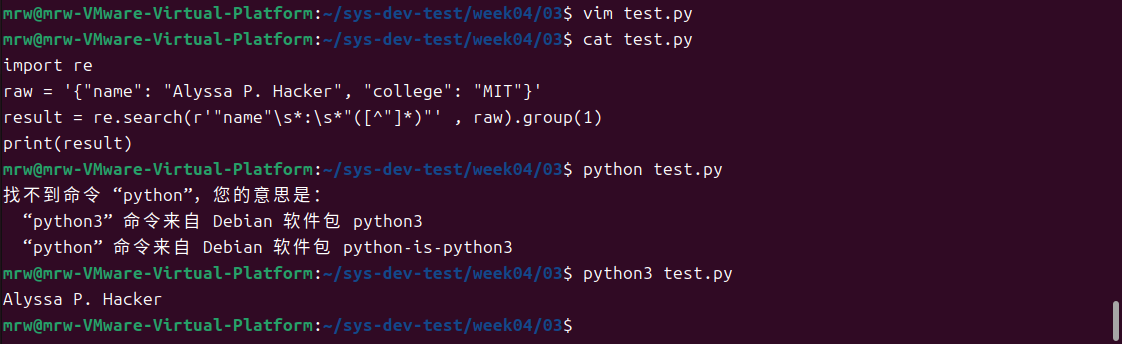
\includegraphics[width=\textwidth]{work04-3.png}
        \caption{用非贪婪捕获组提取 JSON 中的 name}
        \label{work04-3}
      \end{figure}
    \subsection{第04题}
      \subsubsection{题目描述}
      让第3题所写的这个 regex 模式在 name 中包含 " 字符时也能工作（在 JSON 中，双引号可以用 \" 转义）。
      \subsubsection{解题步骤}
      在上题的基础上把捕获组改为 \detokenize{"name"\s*:\s*"((?:[^"\\]|\\.)*)"}：其中 \detokenize{(?:[^"\\]|\\.)} 表示“一个非引号且非反斜杠的字符”或“一个反斜杠后跟任意字符”的序列，因此遇到被转义的 \detokenize{\"} 时不会提前终止匹配。以 \detokenize{raw = r'{"name": "Alyssa P. \"Hacker", "college": "MIT"}'} 为输入，执行 python3 test.py 输出 \detokenize{Alyssa P. \"Hacker}。
      \noindent
      \begin{figure}[H]
        \centering
        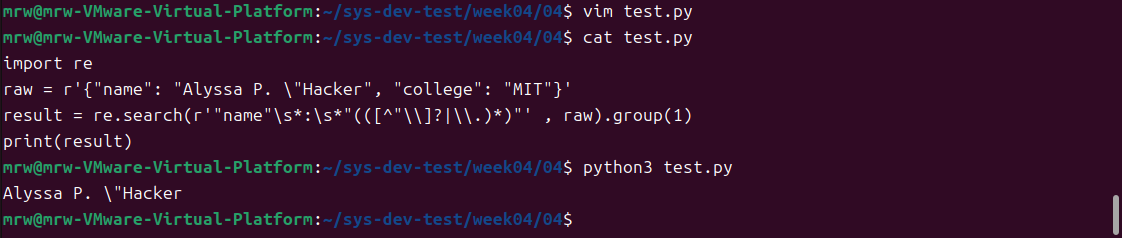
\includegraphics[width=\textwidth]{work04-4.png}
        \caption{兼容转义引号的正则表达式}
        \label{work04-4}
      \end{figure}
    \subsection{第05题}
      \subsubsection{题目描述}
      写一个命令行程序，从标准输入读取第三题上述形式的 JSON 结构，并把 name 输出到标准输出。你应该只需要几行代码就能完成。在 Python 中，除了 import json 之外，一行代码就可以轻松做到。
      \subsubsection{解题步骤}
      在 05 目录下新建 test.py，仅需两行代码：先 \detokenize{import json, sys}，再用 \detokenize{print(json.load(sys.stdin)['name'])} 从标准输入读取 JSON 并输出 name。将第 3 题形式的 JSON 传入，执行 python3 test.py 输出 Alyssa P. Hacker。可以发现直接调用 json 模块解析相较于手写正则表达式更可靠。
      \noindent
      \begin{figure}[H]
        \centering
        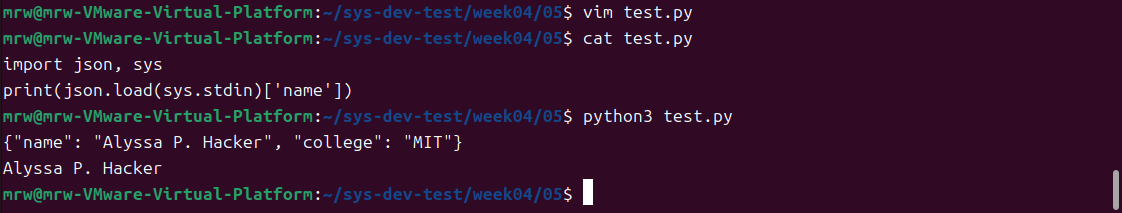
\includegraphics[width=\textwidth]{work04-5.png}
        \caption{从标准输入读取 JSON 并输出 name}
        \label{work04-5}
      \end{figure}
    \subsection{第06题}
      \subsubsection{题目描述}
      大多数的 makefiles 都提供了 一个名为 clean 的构建目标，这并不是说我们会生成一个名为 clean 的文件，而是我们可以使用它清理文件，让 make 重新构建。您可以理解为它的作用是“撤销”所有构建步骤。在上面（2020年课程资料的“元编程”的示例）的 makefile 中为 paper.pdf 实现一个 clean 目标。您需要将构建目标设置为 phony。您也许会发现 git ls-files 子命令很有用。
      \subsubsection{解题步骤}
      首先根据课程讲义补齐构建所需的文件。 Makefile 中 paper.pdf 依赖 paper.tex 与 plot-data.png，中间产物 plot-data.png 由 plot.py 从 data.dat 生成，故先给 plot.py 添加执行权限并用 git init 记录源文件。随后为 paper.pdf 添加 clean 目标并声明为 phony。执行 clean 命令时先用 rm -f paper.pdf 删除最终产物，再用 \detokenize{git ls-files --others --exclude-standard} 列出所有未被 Git 跟踪且未被忽略的文件（即构建产生的中间文件）并一并删除。执行 make paper.pdf 成功生成产物，ls 与 make clean 验证 clean 目标是否只删除产物而保留源文件。
      \noindent
      \begin{figure}[H]
        \centering
        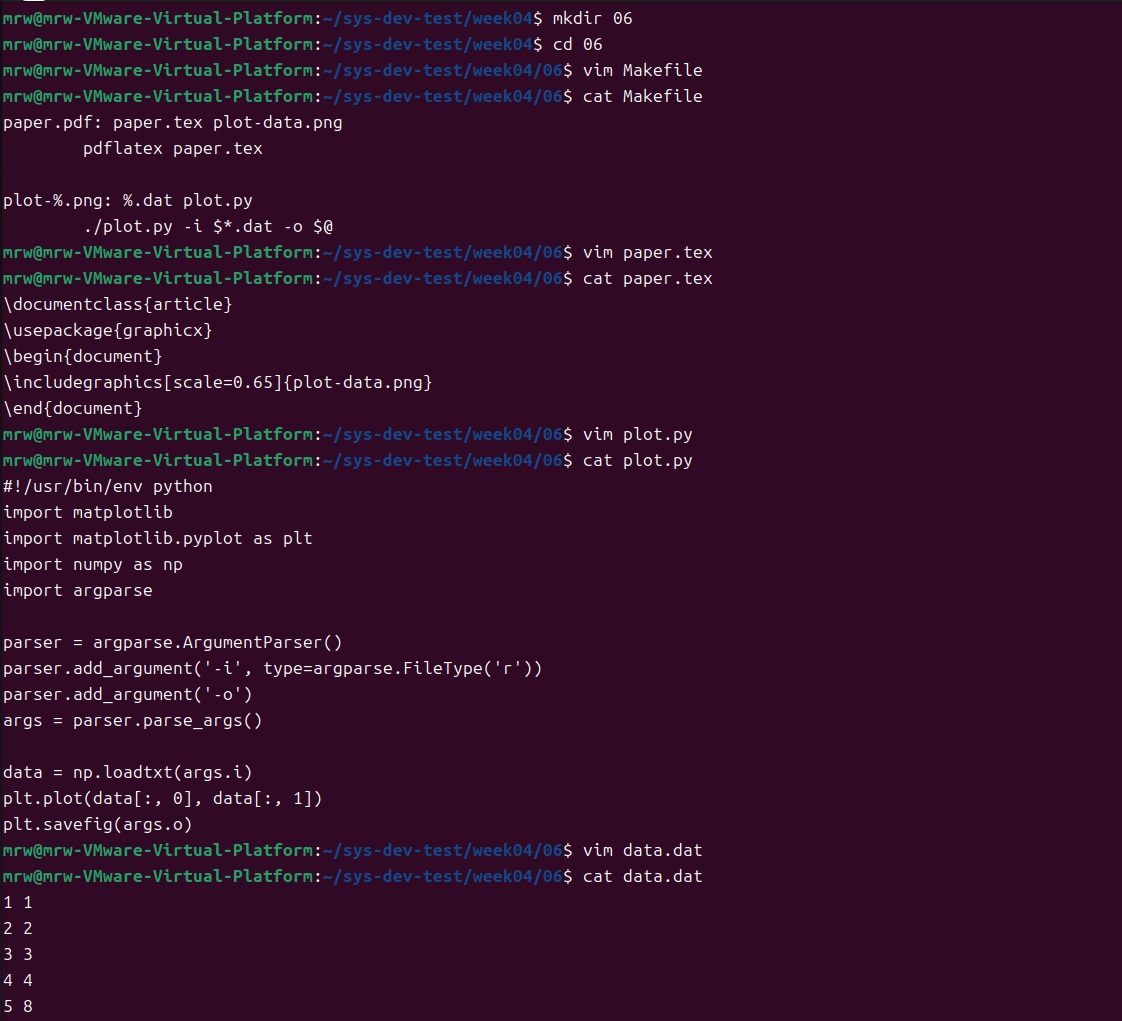
\includegraphics[width=\textwidth]{work04-6-1.png}
        \caption{创建 Makefile、paper.tex、plot.py 与 data.dat}
        \label{work04-6-1}
      \end{figure}
      \noindent
      \begin{figure}[H]
        \centering
        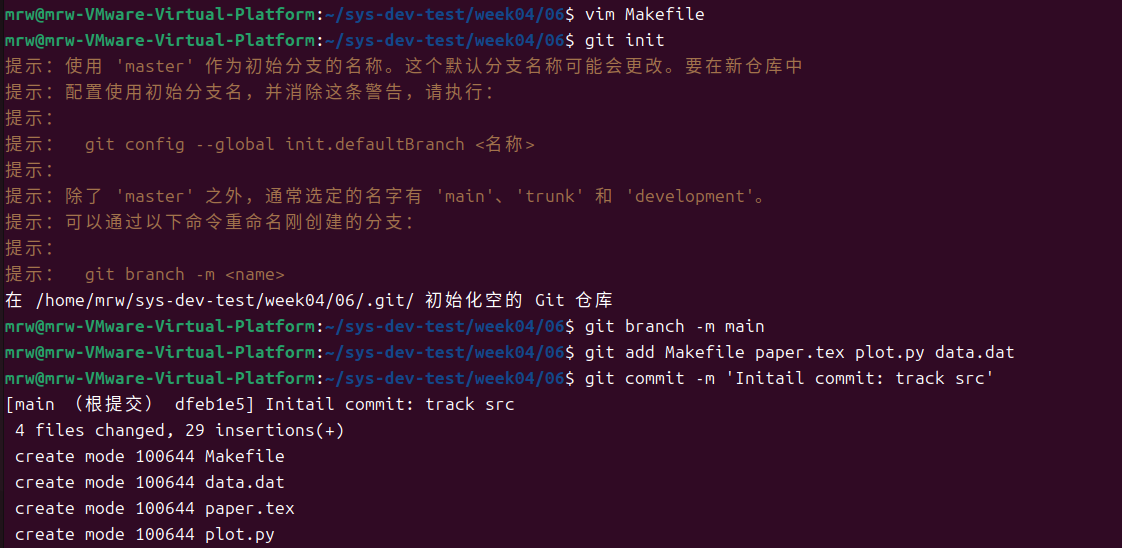
\includegraphics[width=\textwidth]{work04-6-2.png}
        \caption{添加 clean 目标并初始化 Git 仓库}
        \label{work04-6-2}
      \end{figure}
      \noindent
      \begin{figure}[H]
        \centering
        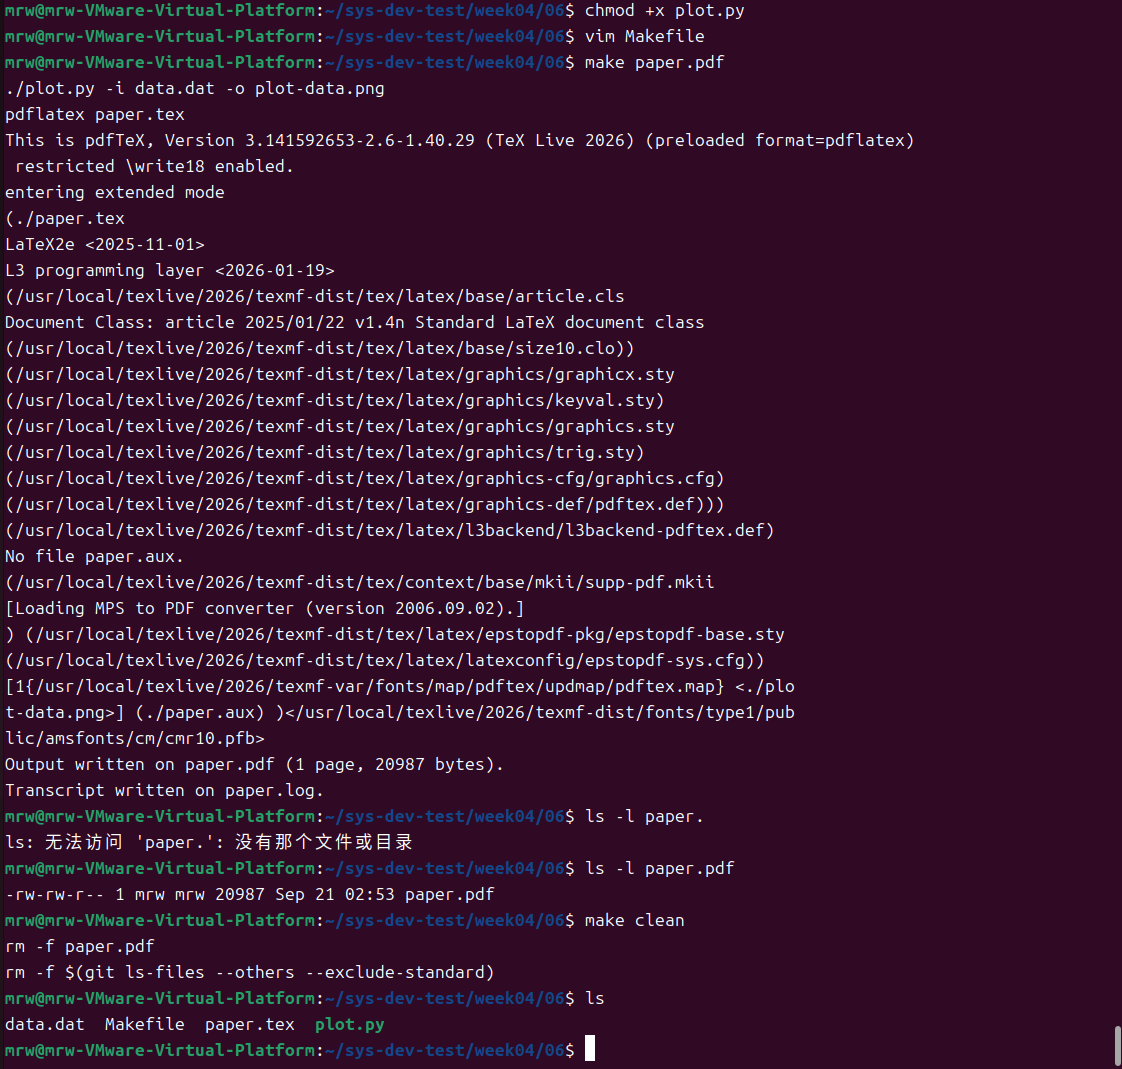
\includegraphics[width=\textwidth]{work04-6-3.png}
        \caption{make paper.pdf 与 make clean 的执行结果}
        \label{work04-6-3}
      \end{figure}
    \subsection{第07题}
      \subsubsection{题目描述}
      Git 可以作为一个简单的 CI 系统来使用，在任何 git 仓库中的 .git/hooks 目录中，您可以找到一些文件（当前处于未激活状态），它们的作用和脚本一样，当某些事件发生时便可以自动执行。请编写一个 pre-commit 钩子，它会在提交前执行 make paper.pdf 并在出现构建失败的情况拒绝您的提交。
      \subsubsection{解题步骤}
      在 .git/hooks 下新建 pre-commit 钩子并赋予执行权限，pre-commit 先执行 \detokenize{make paper.pdf}，若构建失败则打印 Build failed. Commit rejected. 并以退出码 1 中止提交。用 git add . 将原先的 4 个文件加入缓存区随后提交，pre-commit 执行构建成功后提交正常完成。再把 paper.tex 中的图片改为不存在的 plot-nonexist.png 后再次提交，pdflatex 因找不到该文件报错，make 返回非零状态码，pre-commit 输出 Build failed. Commit rejected. 并拒绝该次提交。
      \noindent
      \begin{figure}[H]
        \centering
        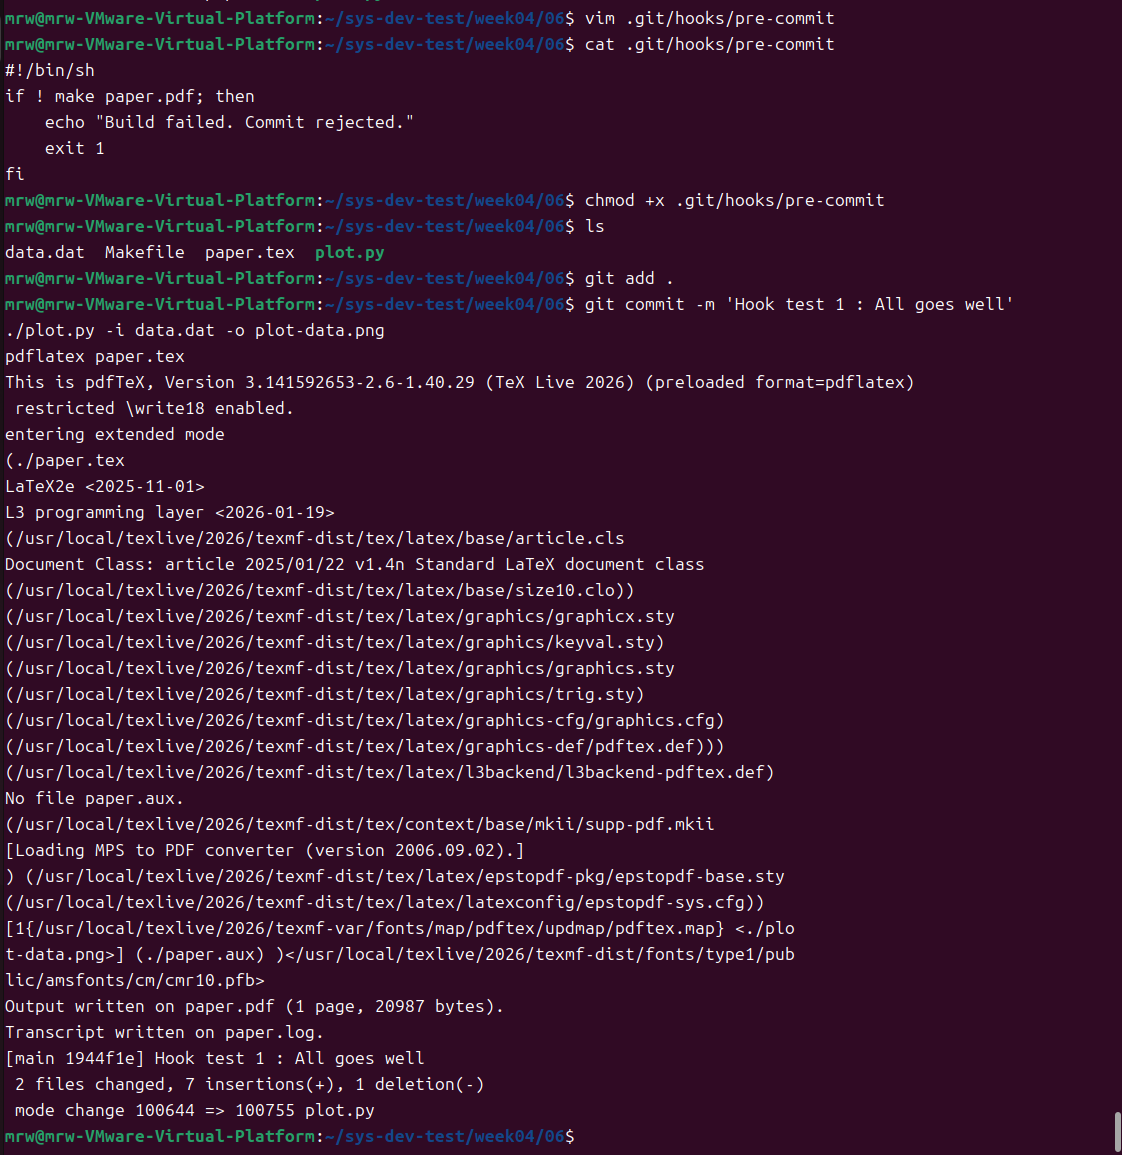
\includegraphics[width=\textwidth]{work04-7-1.png}
        \caption{编写 pre-commit 钩子并成功提交}
        \label{work04-7-1}
      \end{figure}
      \noindent
      \begin{figure}[H]
        \centering
        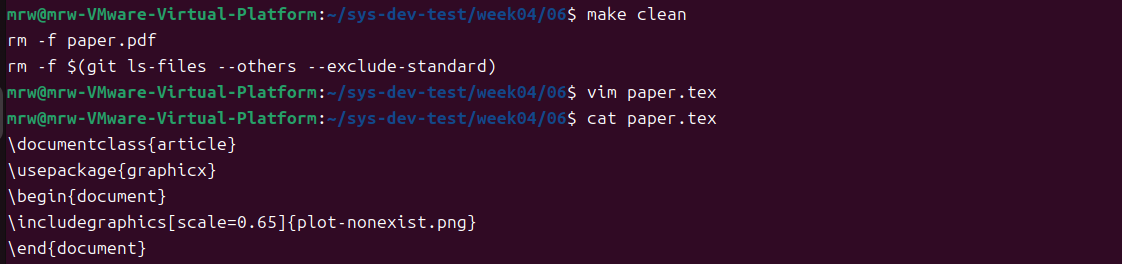
\includegraphics[width=\textwidth]{work04-7-2.png}
        \caption{清理产物并把图片改为不存在的文件}
        \label{work04-7-2}
      \end{figure}
      \noindent
      \begin{figure}[H]
        \centering
        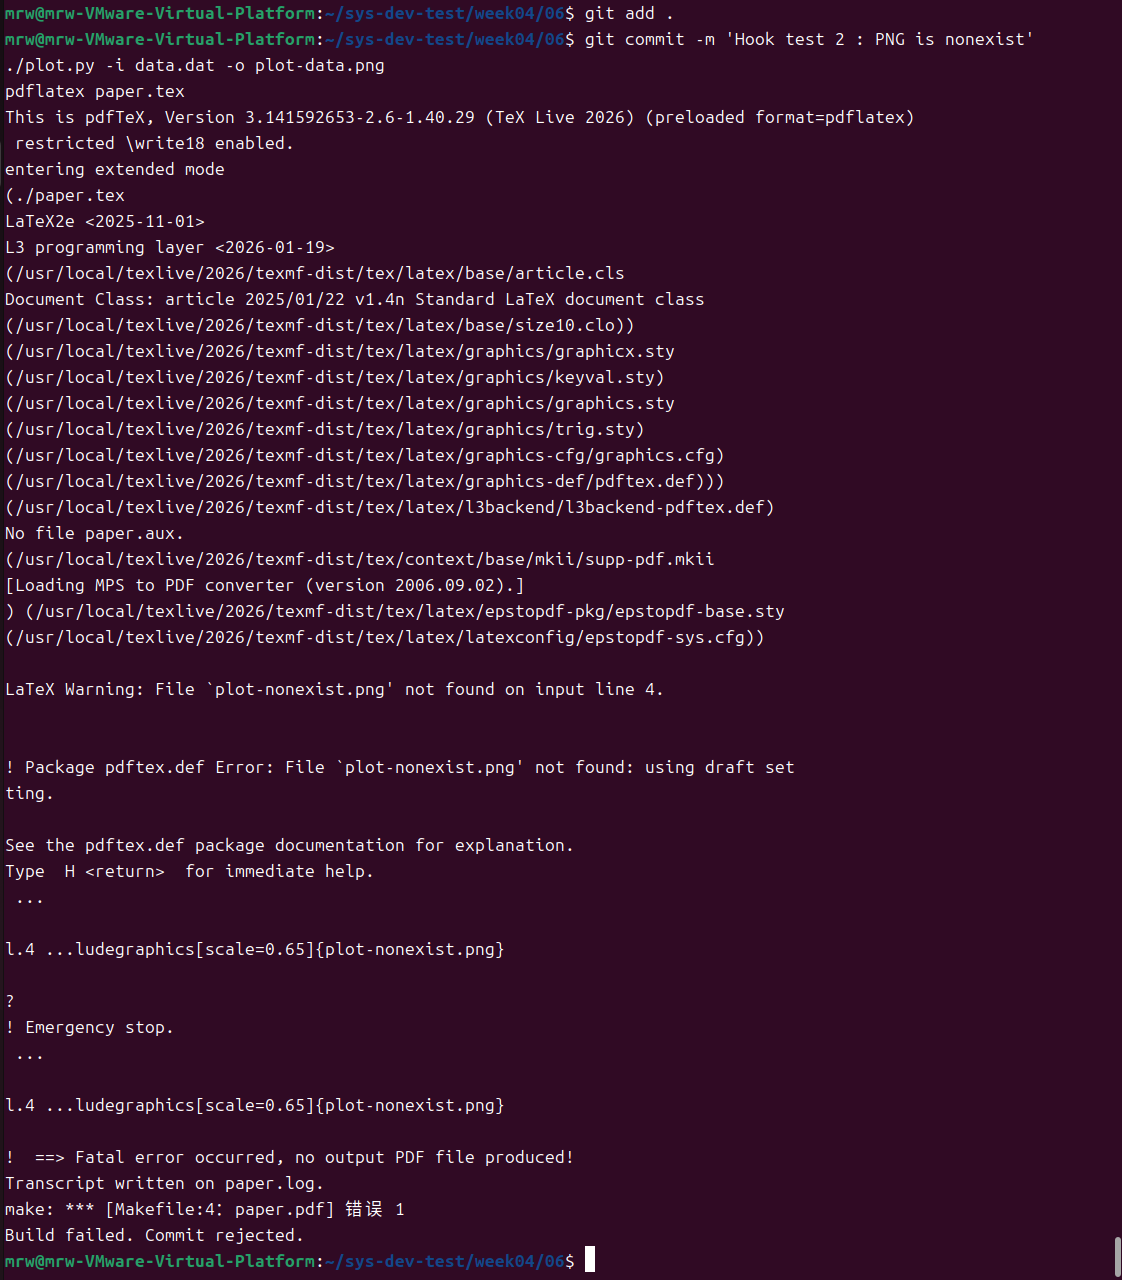
\includegraphics[width=\textwidth]{work04-7-3.png}
        \caption{构建失败导致提交被拒绝}
        \label{work04-7-3}
      \end{figure}
    \subsection{第08题}
      \subsubsection{题目描述}
      学习一下 Rust 的构建系统的依赖管理，对于每种语法(尖号、波浪号、通配符、比较、多个版本要求)，构建一种场景使其具有实际意义。
      \subsubsection{解题步骤}
      \begin{itemize}
      \item \textbf{尖号（\textasciicircum{}）}：\textasciicircum{}1.2.3 等价于 $\ge$1.2.3, $<$2.0.0。适用于希望自动获得向后兼容的新功能，例如 \textasciicircum{}1.2.3 允许升级到 1.9.0，但不会升级到 2.0.0。
      \item \textbf{波浪号（\textasciitilde{}）}：\textasciitilde{}1.2.3 允许升级到 1.2.x（x $\ge$ 3），但不会改变次版本号。适用于需要特定次版本系列内的补丁更新。
      \item \textbf{通配符（*）}：1.* 匹配所有 1.x.y 版本。适用于内部工具，不关心具体版本，只要主版本号一致即可。
      \item \textbf{比较（$>$、$<$）}：$>$1.2.3 或 $<$2.0.0。适用于需要严格限定版本范围的场景，例如避开某个已知有问题的版本。
      \item \textbf{多个版本要求}：用逗号分隔，如 $\ge$1.2.0, $<$1.5.0。适用于需要同时满足多个约束条件的场景。
      \end{itemize}
      \noindent
    \subsection{第09题}
      \subsubsection{题目描述}
      基于 GitHub Pages 创建任意一个可以自动发布的页面。添加一个 GitHub Action 到该仓库，对仓库中的所有 shell 文件执行 shellcheck。
      \subsubsection{解题步骤}
      先在仓库设置中将 Pages 的 Source 设为 GitHub Actions，并在仓库根目录放置包含“系统开发工具基础”与“这是一个测试页面”的 index.html，发布后可通过 https://mrw1114.github.io/fundamentals-of-system-dev-tools/ 访问。随后在 .github/workflows/blank.yml 中新增工作流，在 push 与 pull\_request 时检查仓库，并用 ludeeus/action-shellcheck 对仓库中所有 shell 文件执行 shellcheck。首次运行失败，报出 SC2148（脚本缺少 shebang）与 SC2086（变量未加双引号）等问题，为相关脚本补上 shebang 并修正引号后再次运行，检查全部通过。
      \noindent
      \begin{figure}[H]
        \centering
        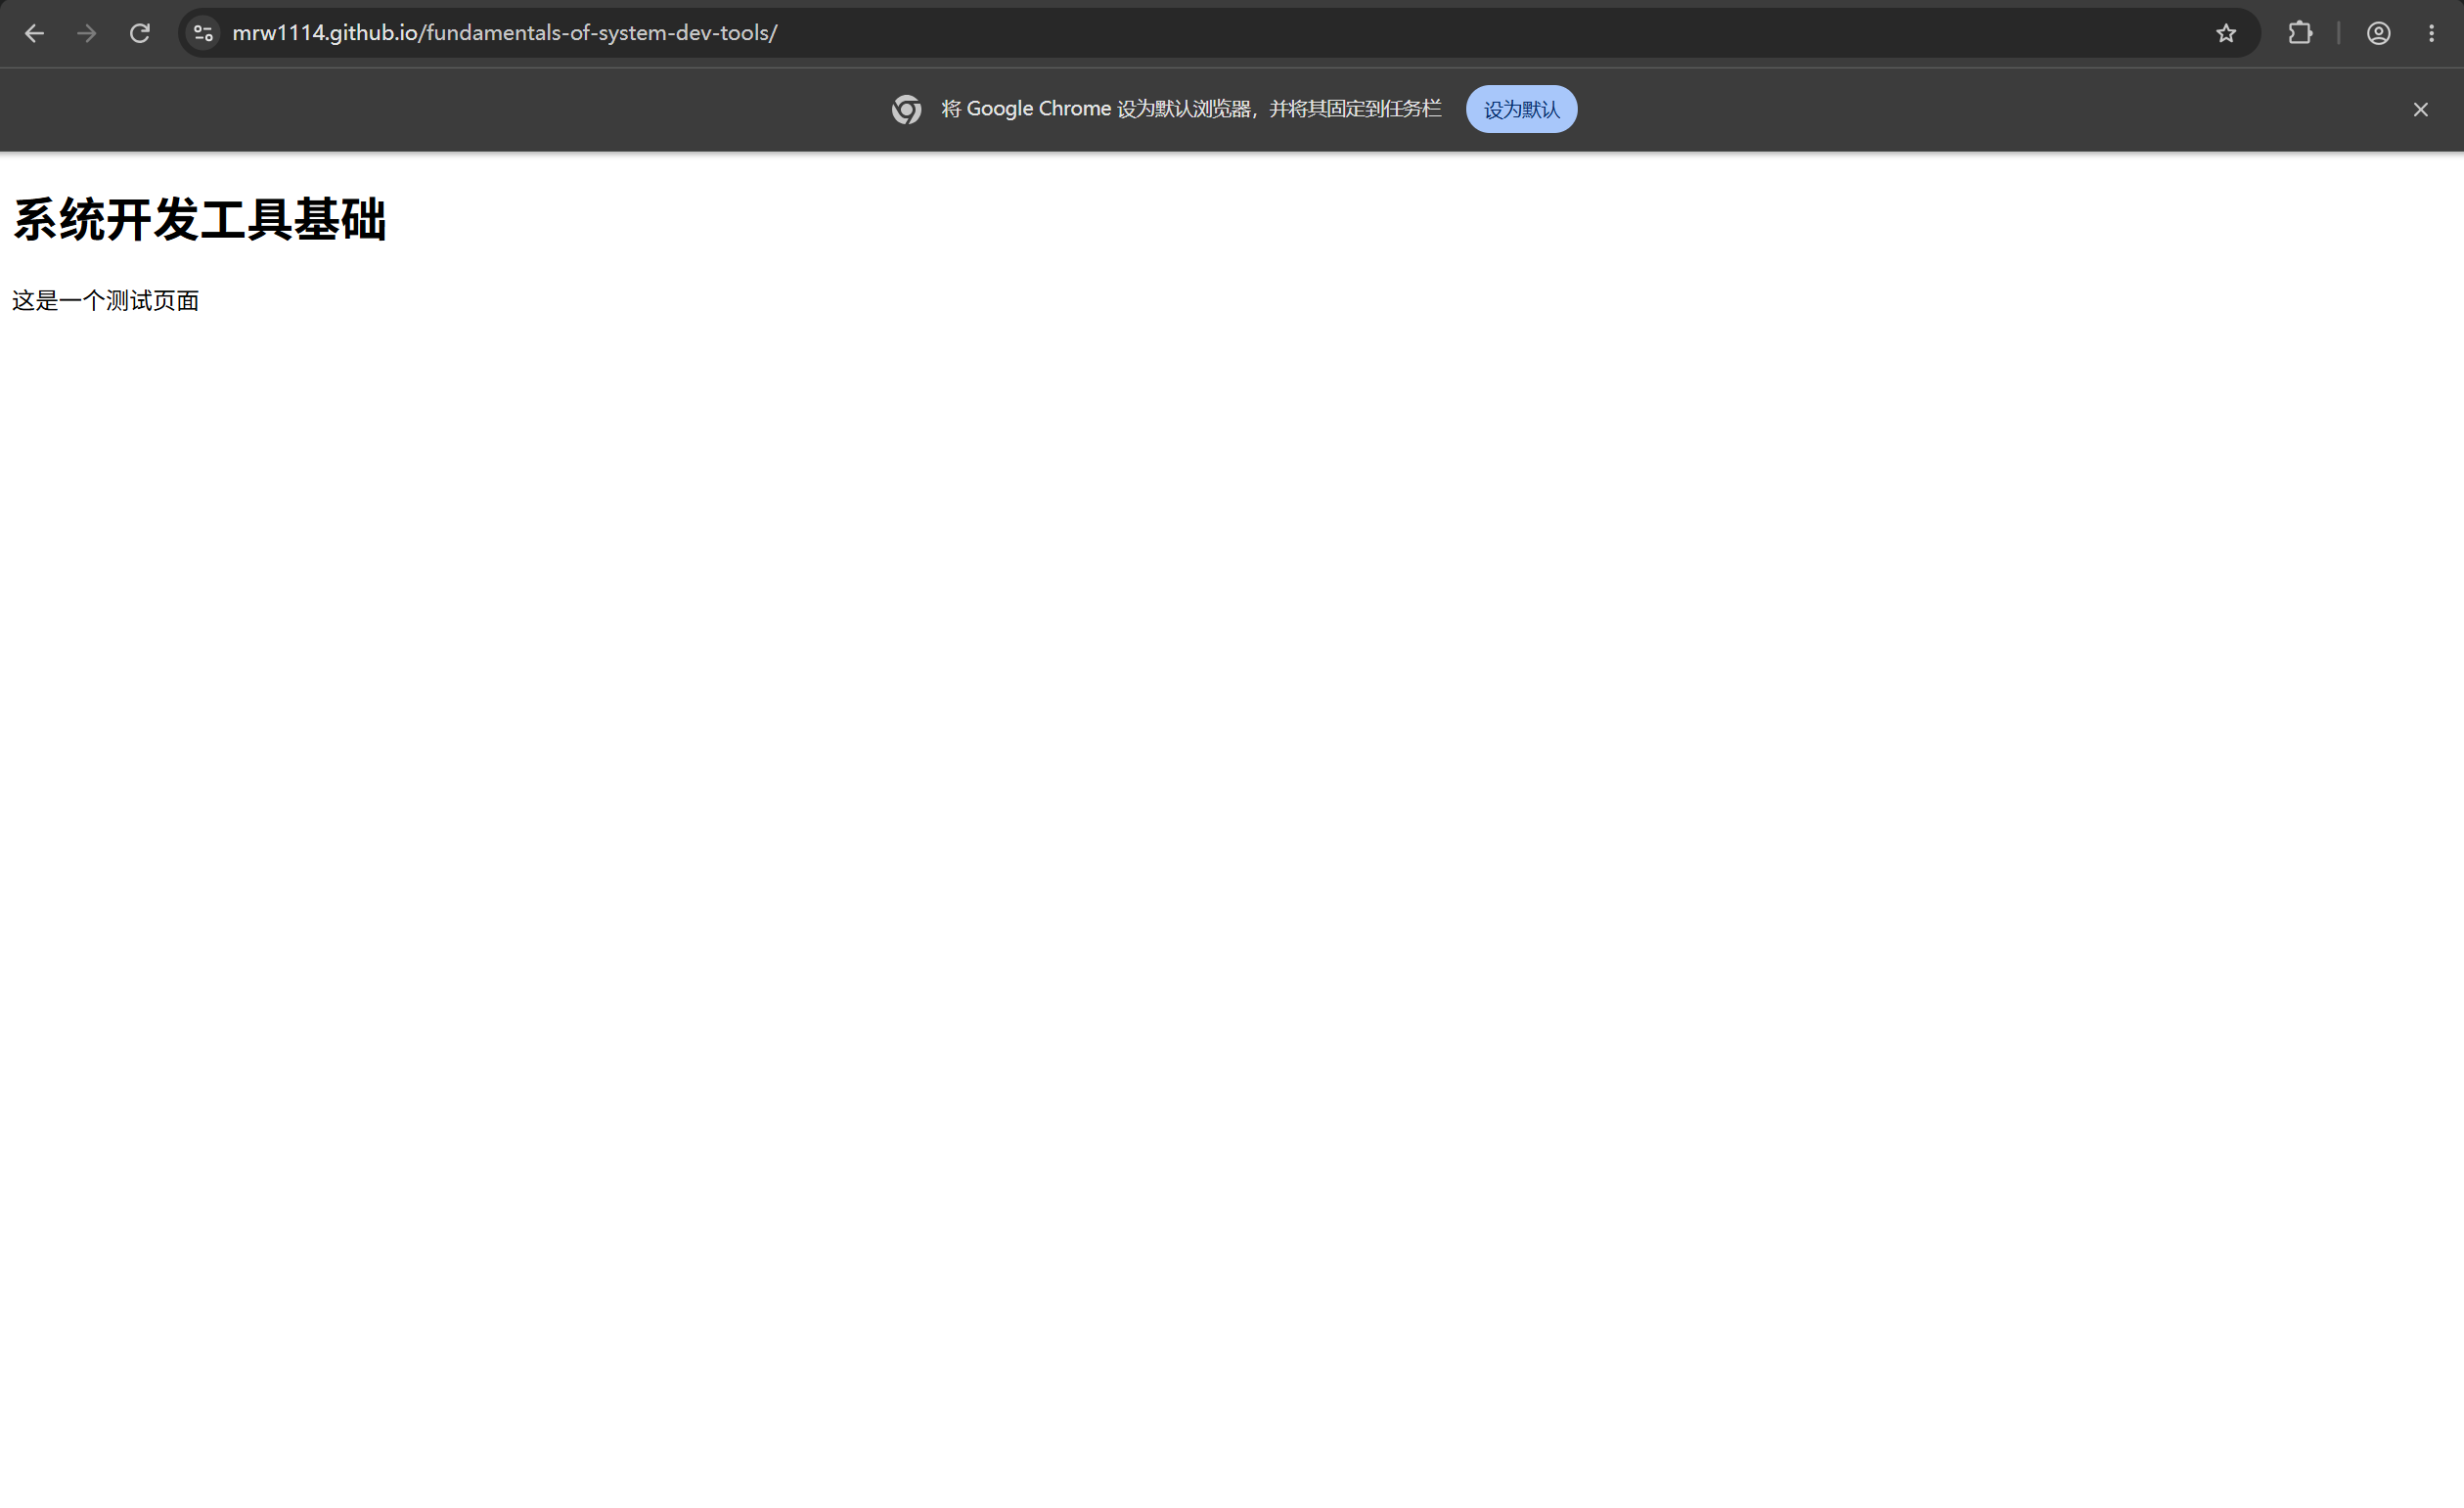
\includegraphics[width=\textwidth]{work04-9-1.png}
        \caption{启用 GitHub Pages 后的测试页面}
        \label{work04-9-1}
      \end{figure}
      \noindent
      \begin{figure}[H]
        \centering
        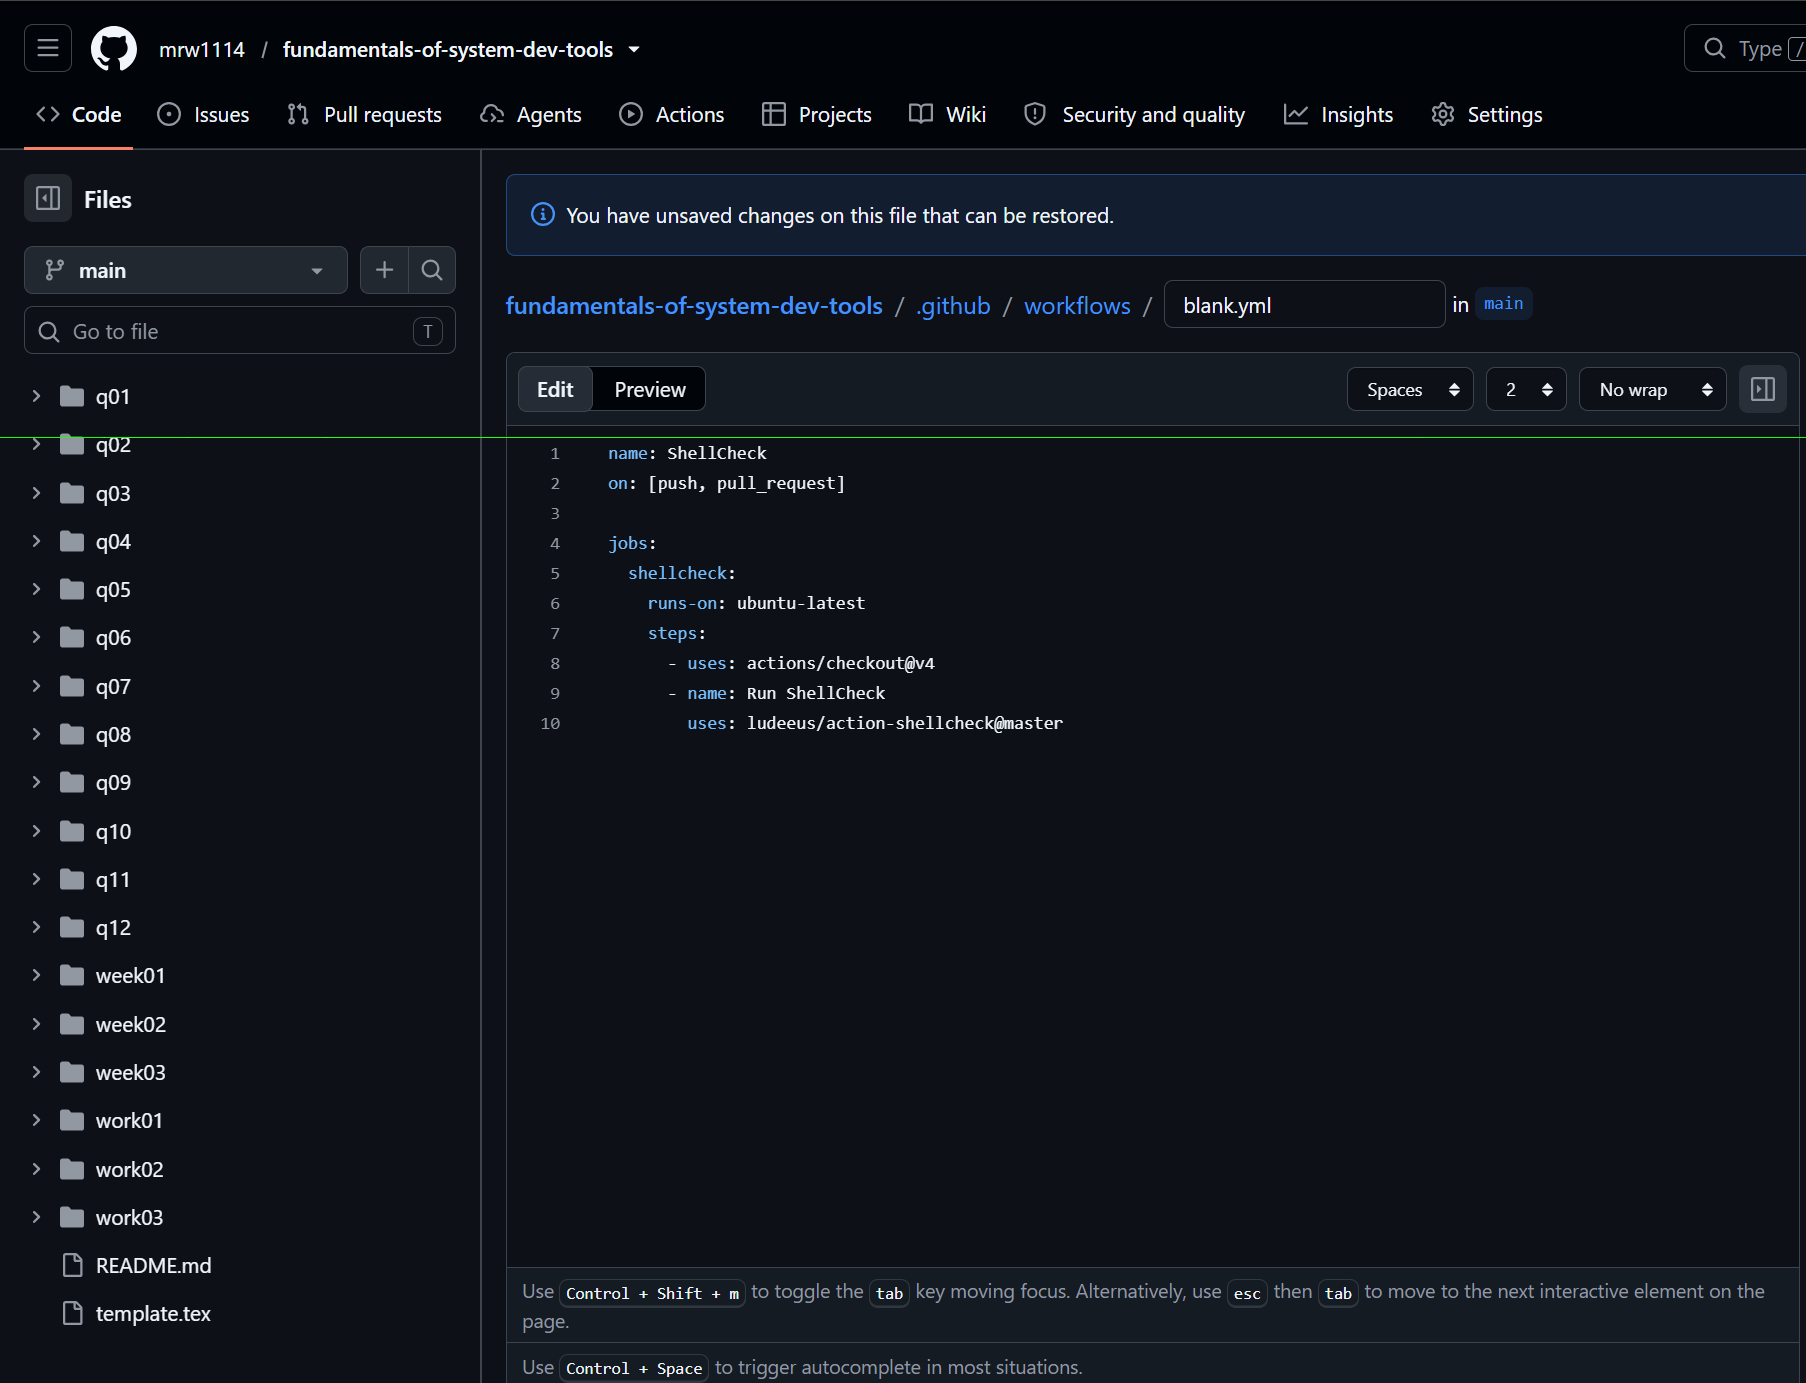
\includegraphics[width=\textwidth]{work04-9-2.png}
        \caption{shellcheck 工作流配置}
        \label{work04-9-2}
      \end{figure}
      \noindent
      \begin{figure}[H]
        \centering
        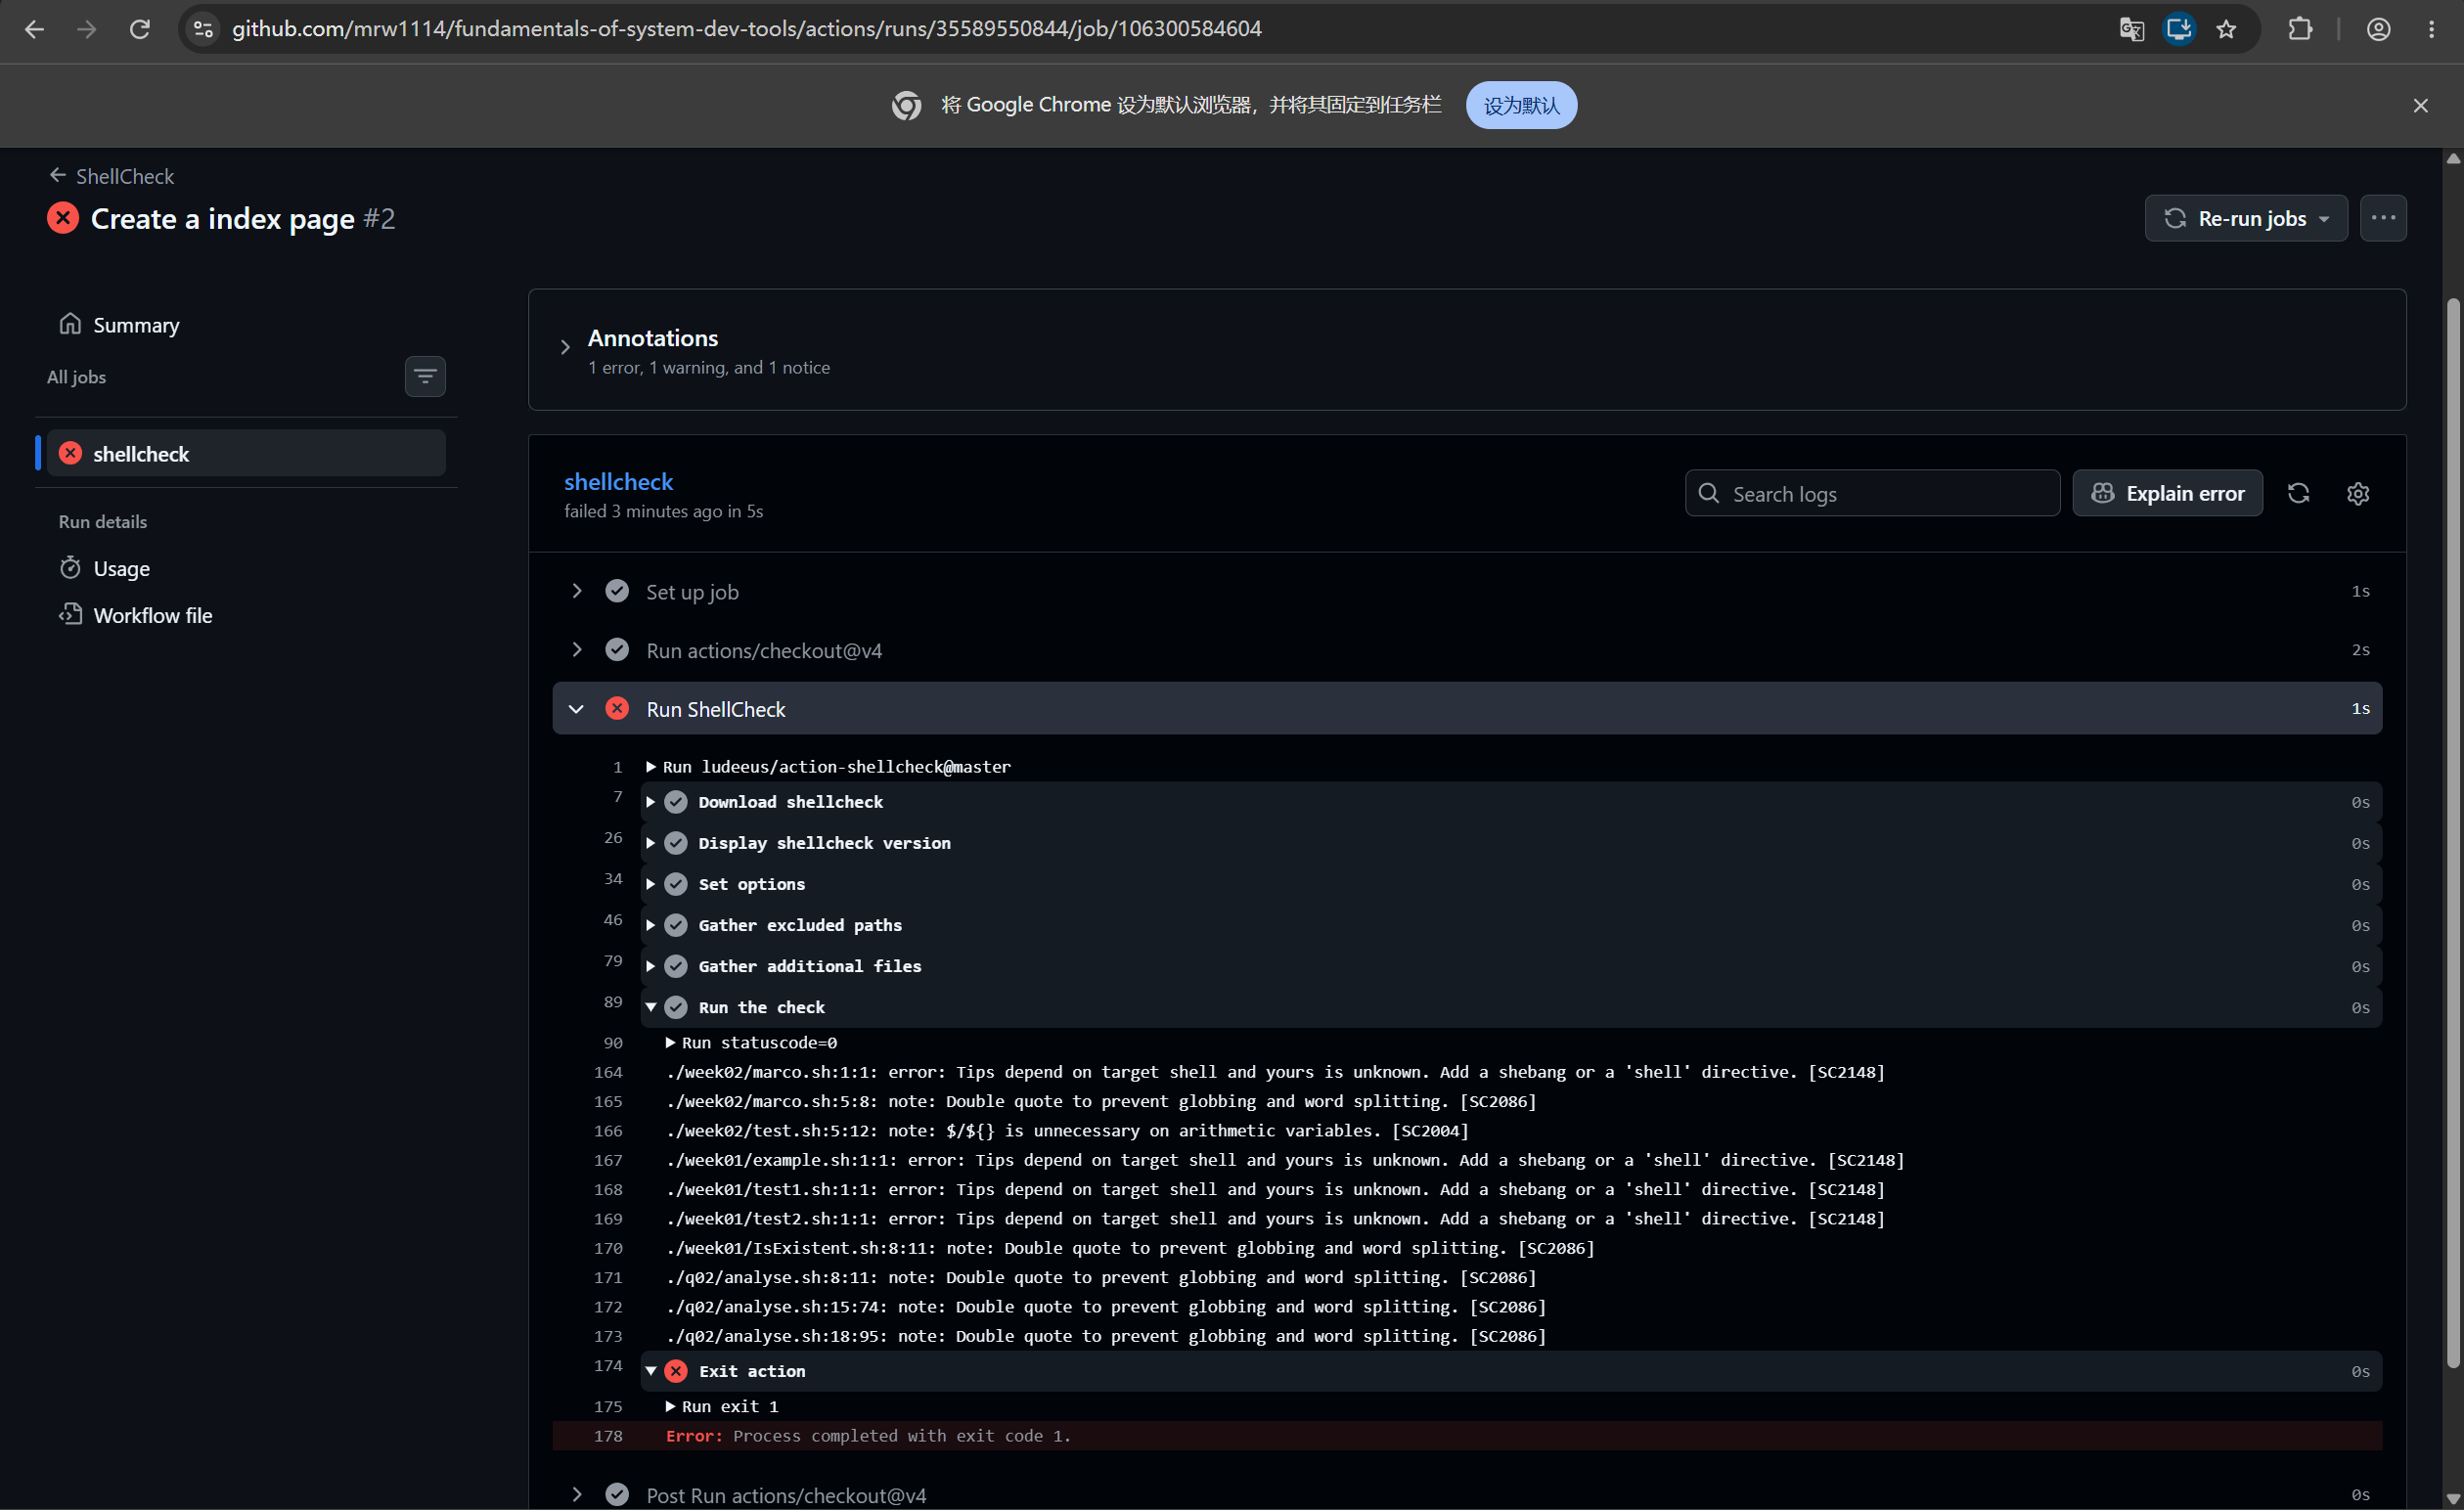
\includegraphics[width=\textwidth]{work04-9-3.png}
        \caption{首次运行报出 SC2148、SC2086 等问题}
        \label{work04-9-3}
      \end{figure}
      \noindent
      \begin{figure}[H]
        \centering
        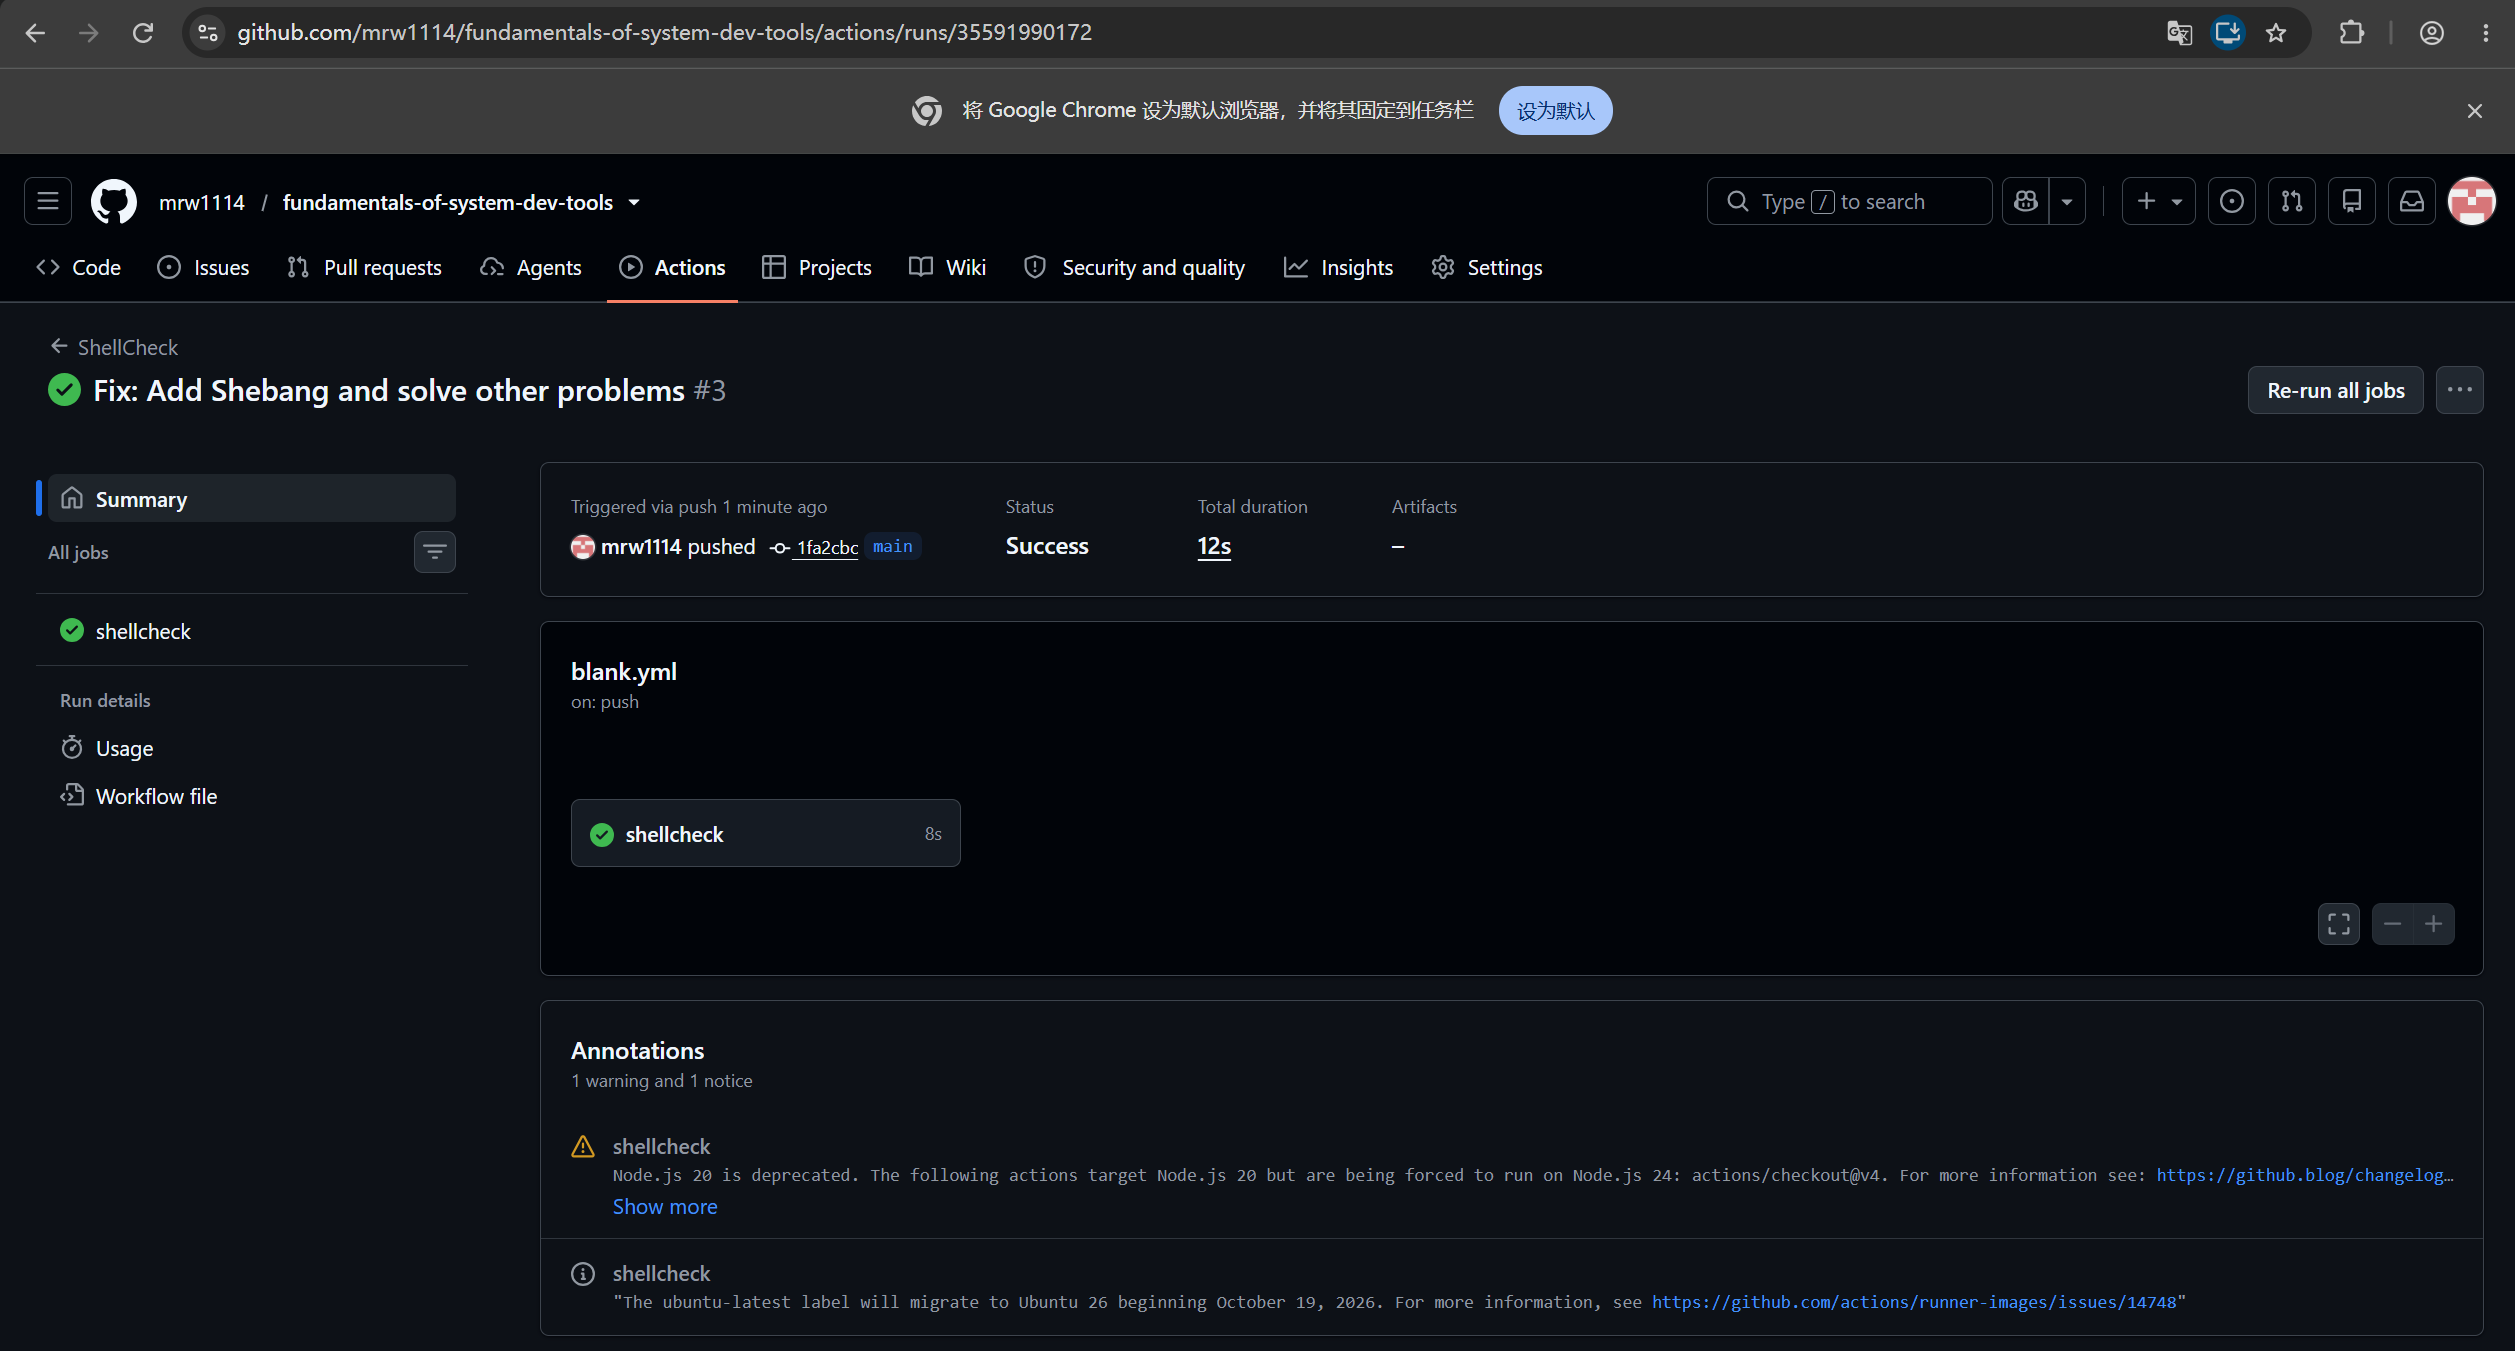
\includegraphics[width=\textwidth]{work04-9-4.png}
        \caption{补充 shebang 并修正后检查通过}
        \label{work04-9-4}
      \end{figure}
    \subsection{第10题}
      \subsubsection{题目描述}
      构建属于您的 GitHub action，对仓库中所有的 .md 文件执行 proselint 或 write-good，在您的仓库中开启这一功能，提交一个包含错误的文件看看该功能是否生效。
      \subsubsection{解题步骤}
      在 .github/workflows/proselint.yml 中新增工作流：在 push 与 pull\_request 时检出仓库、安装 proselint，并用 proselint check \$(git ls-files "*.md") 对仓库中所有 .md 文件执行检查。由于该工具会执行仅涉及写作风格的的双引号和省略号检查，因此在仓库根目录添加 proselintrc.json 并设置相应的忽略规则。在提交后该功能生效并报告 README.md 与 week03/ai\_summary.md 分别报出 lexical\_illusions（词语重复）、annotations.misc（未移除的 TODO 等项目标记） 等错误。修复相关问题后，仓库首页显示包含 Proselint 和 ShellCheck 的5项检查全部通过。
      \noindent
      \begin{figure}[H]
        \centering
        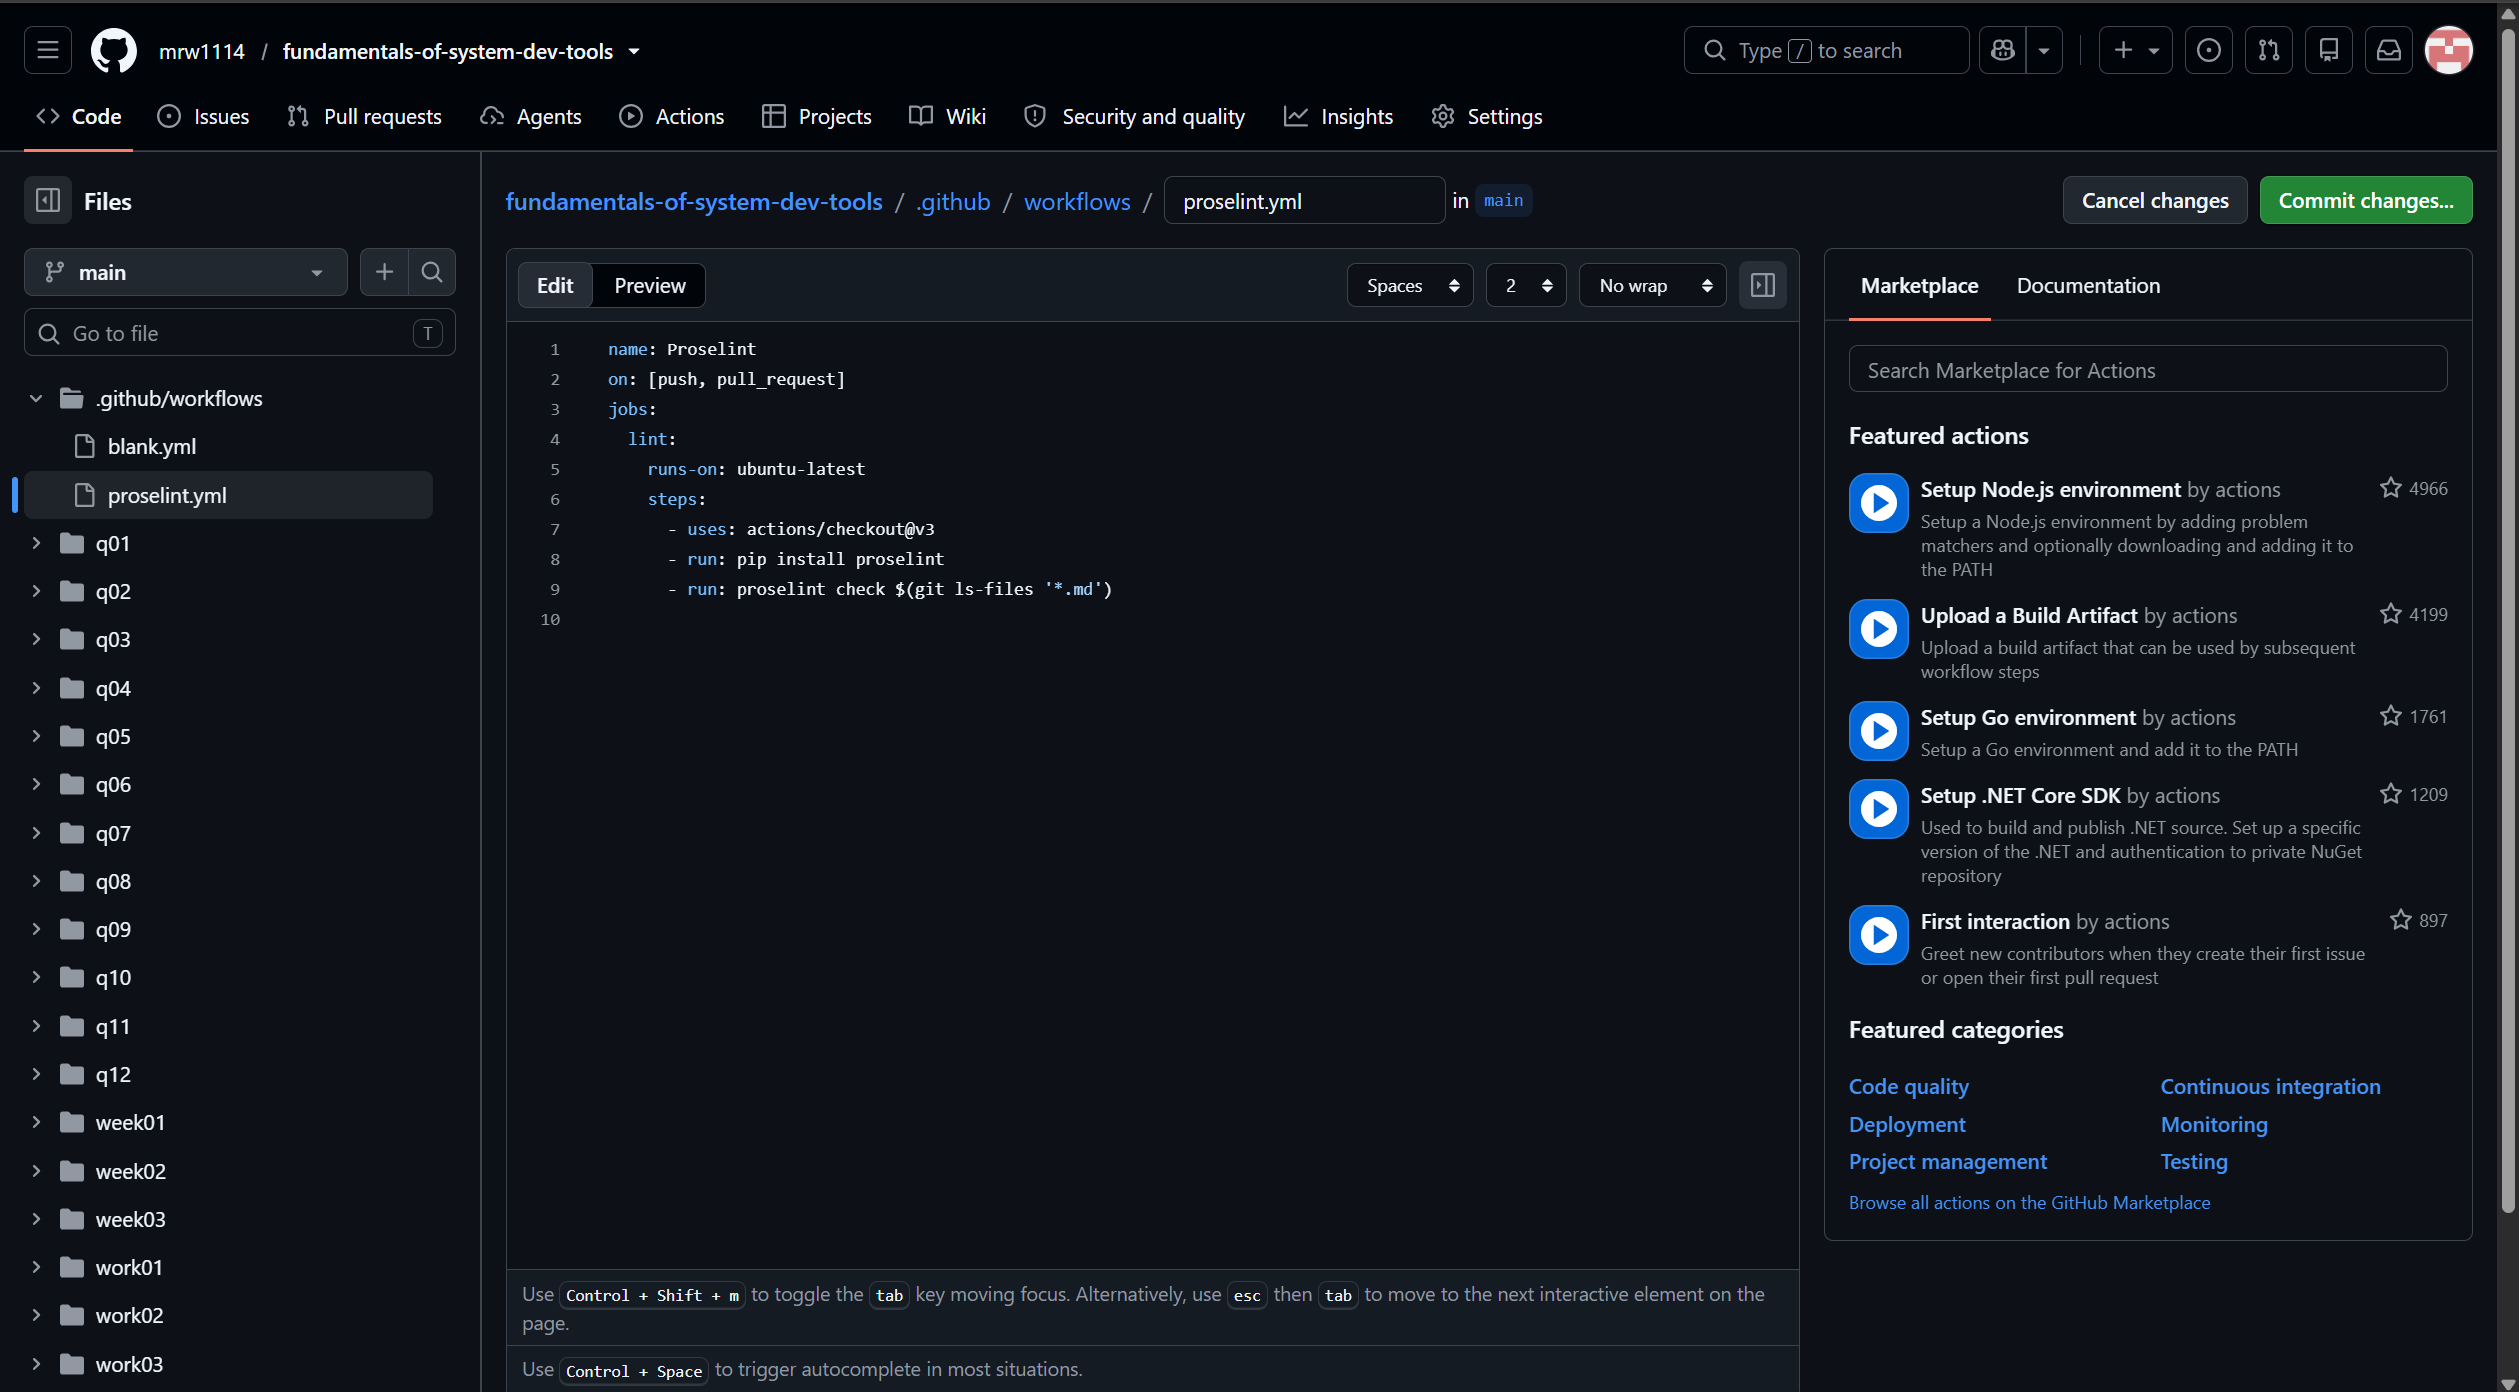
\includegraphics[width=\textwidth]{work04-10-1.png}
        \caption{proselint 工作流配置}
        \label{work04-10-1}
      \end{figure}
      \noindent
      \begin{figure}[H]
        \centering
        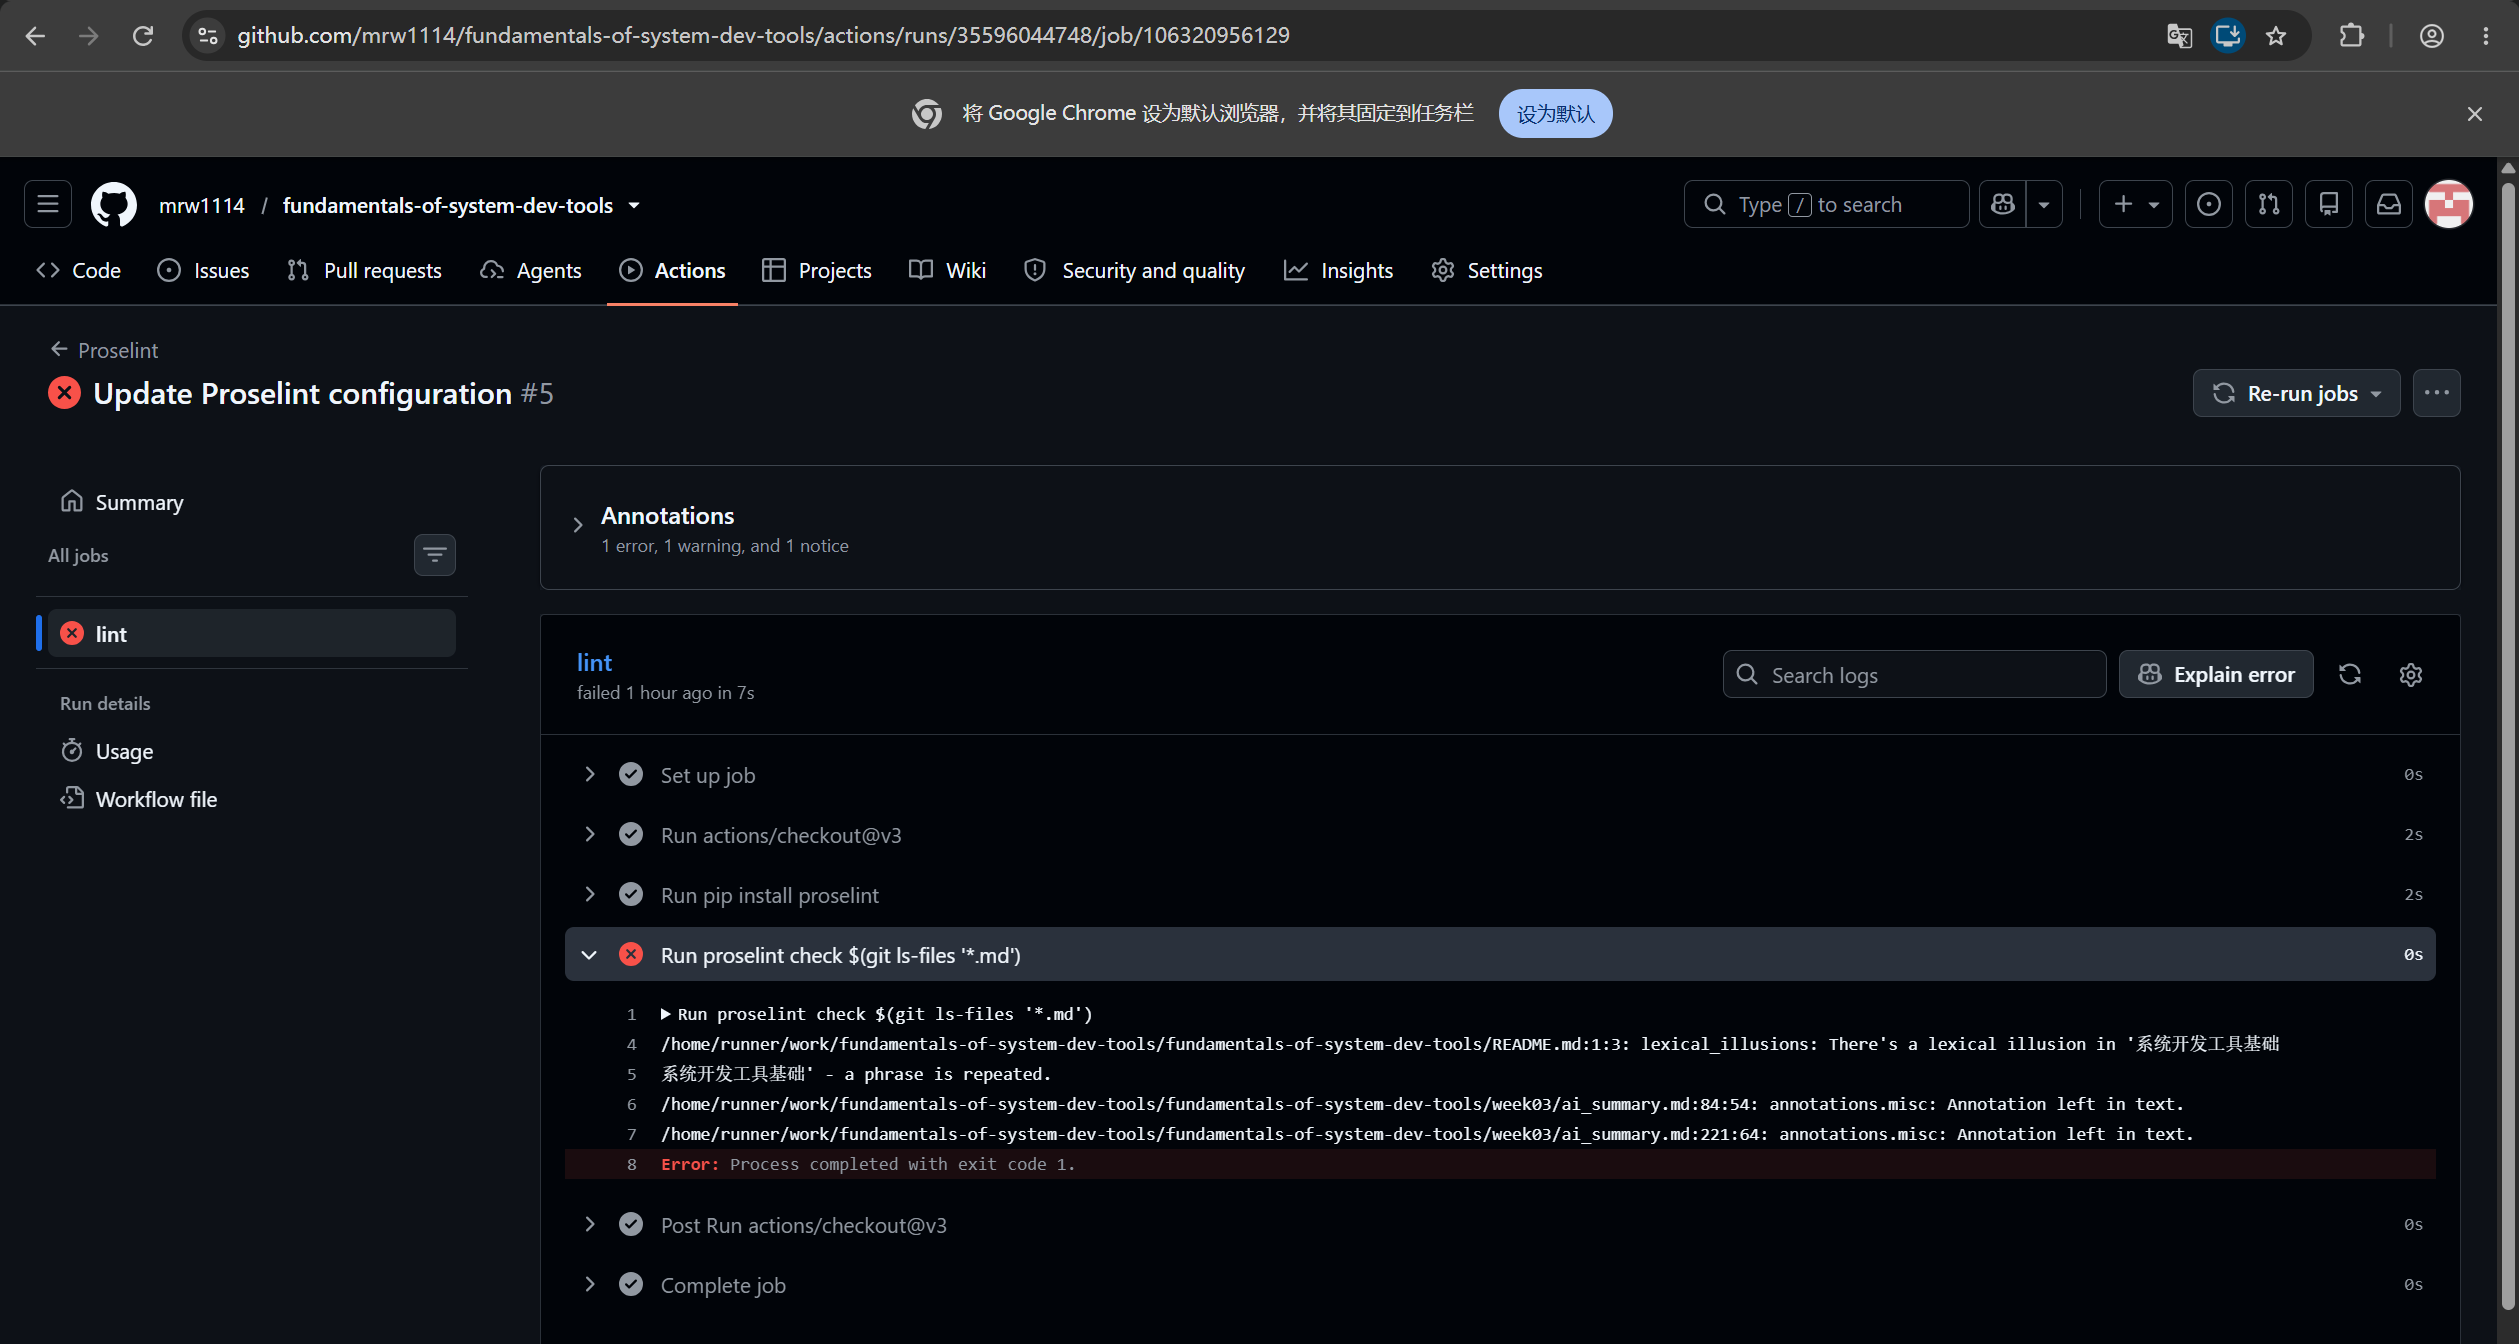
\includegraphics[width=\textwidth]{work04-10-2.png}
        \caption{提交包含错误的文件后检查失败}
        \label{work04-10-2}
      \end{figure}
      \noindent
      \begin{figure}[H]
        \centering
        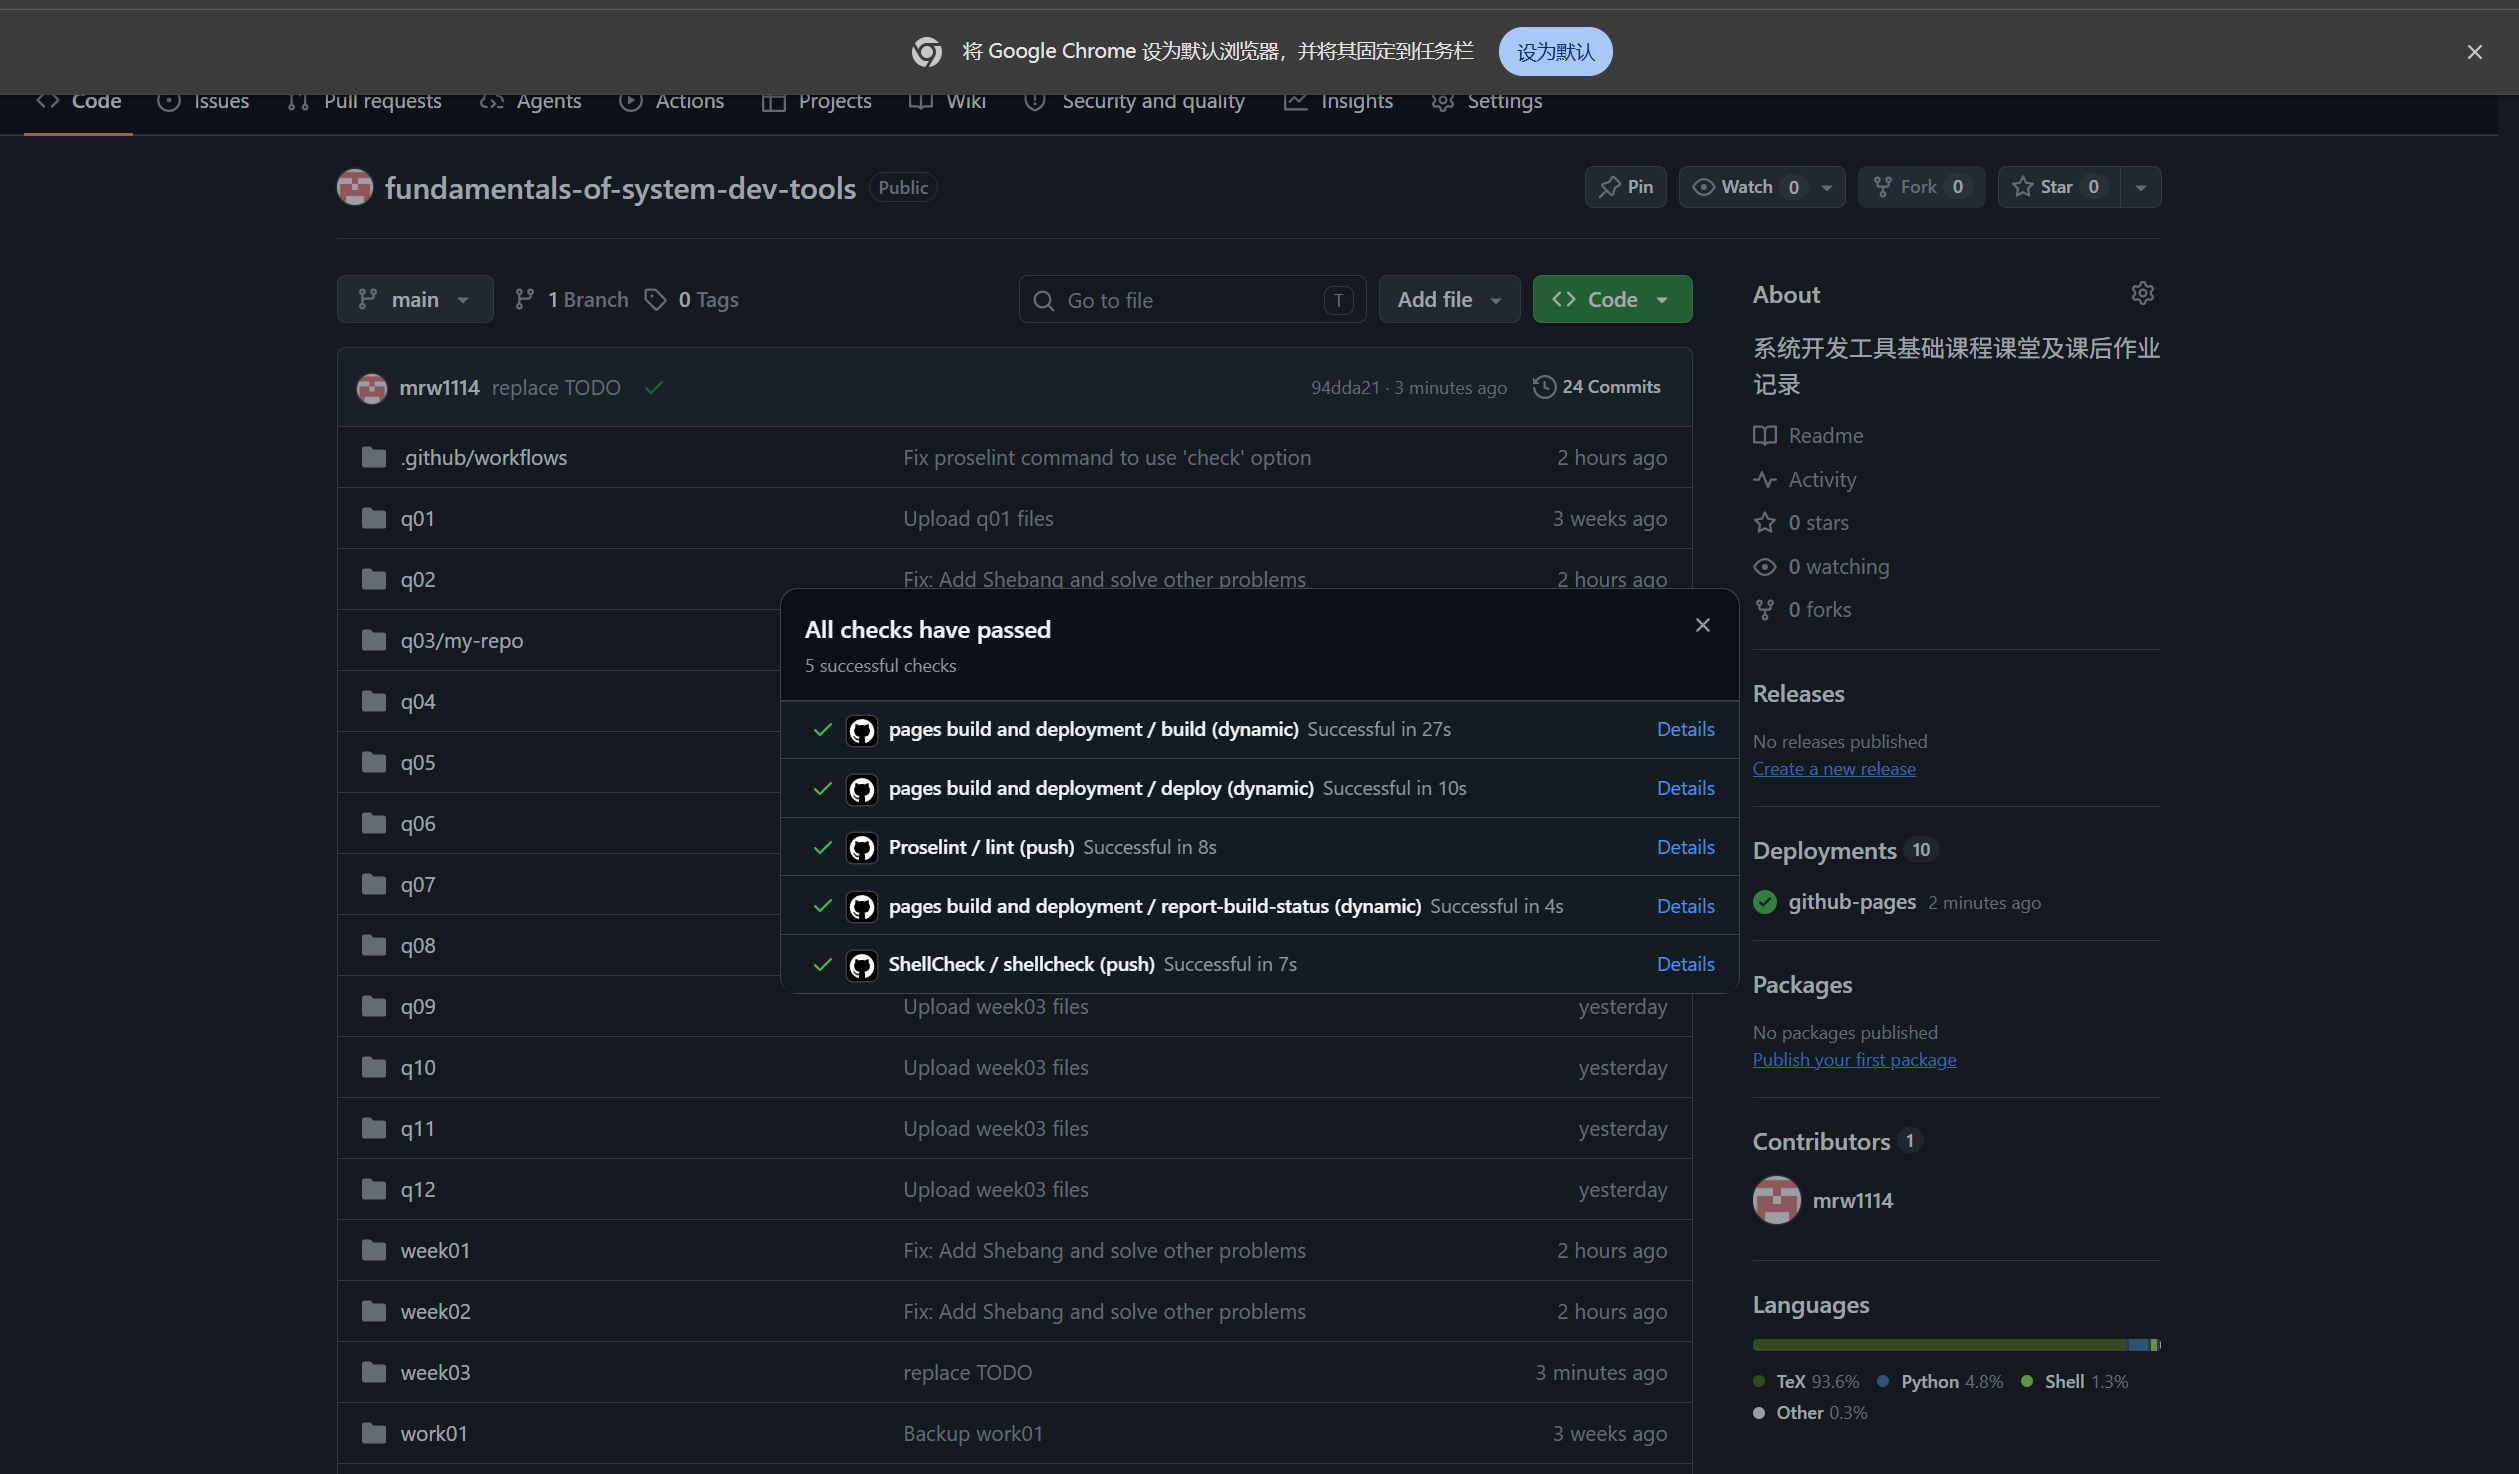
\includegraphics[width=\textwidth]{work04-10-3.png}
        \caption{修复后全部检查通过}
        \label{work04-10-3}
      \end{figure}
  \section{commit 记录}
  \noindent
  commit 记录截图如下，由于课程文件中的 week04/02/code-quality.md 是作业文件但又被 ProseLint 检测，故导致 action 中的检测不通过。后续在配置文件中强行排除该文件后检查通过。详细内容请访问仓库查看。 
      \noindent
      \begin{figure}[H]
        \centering
        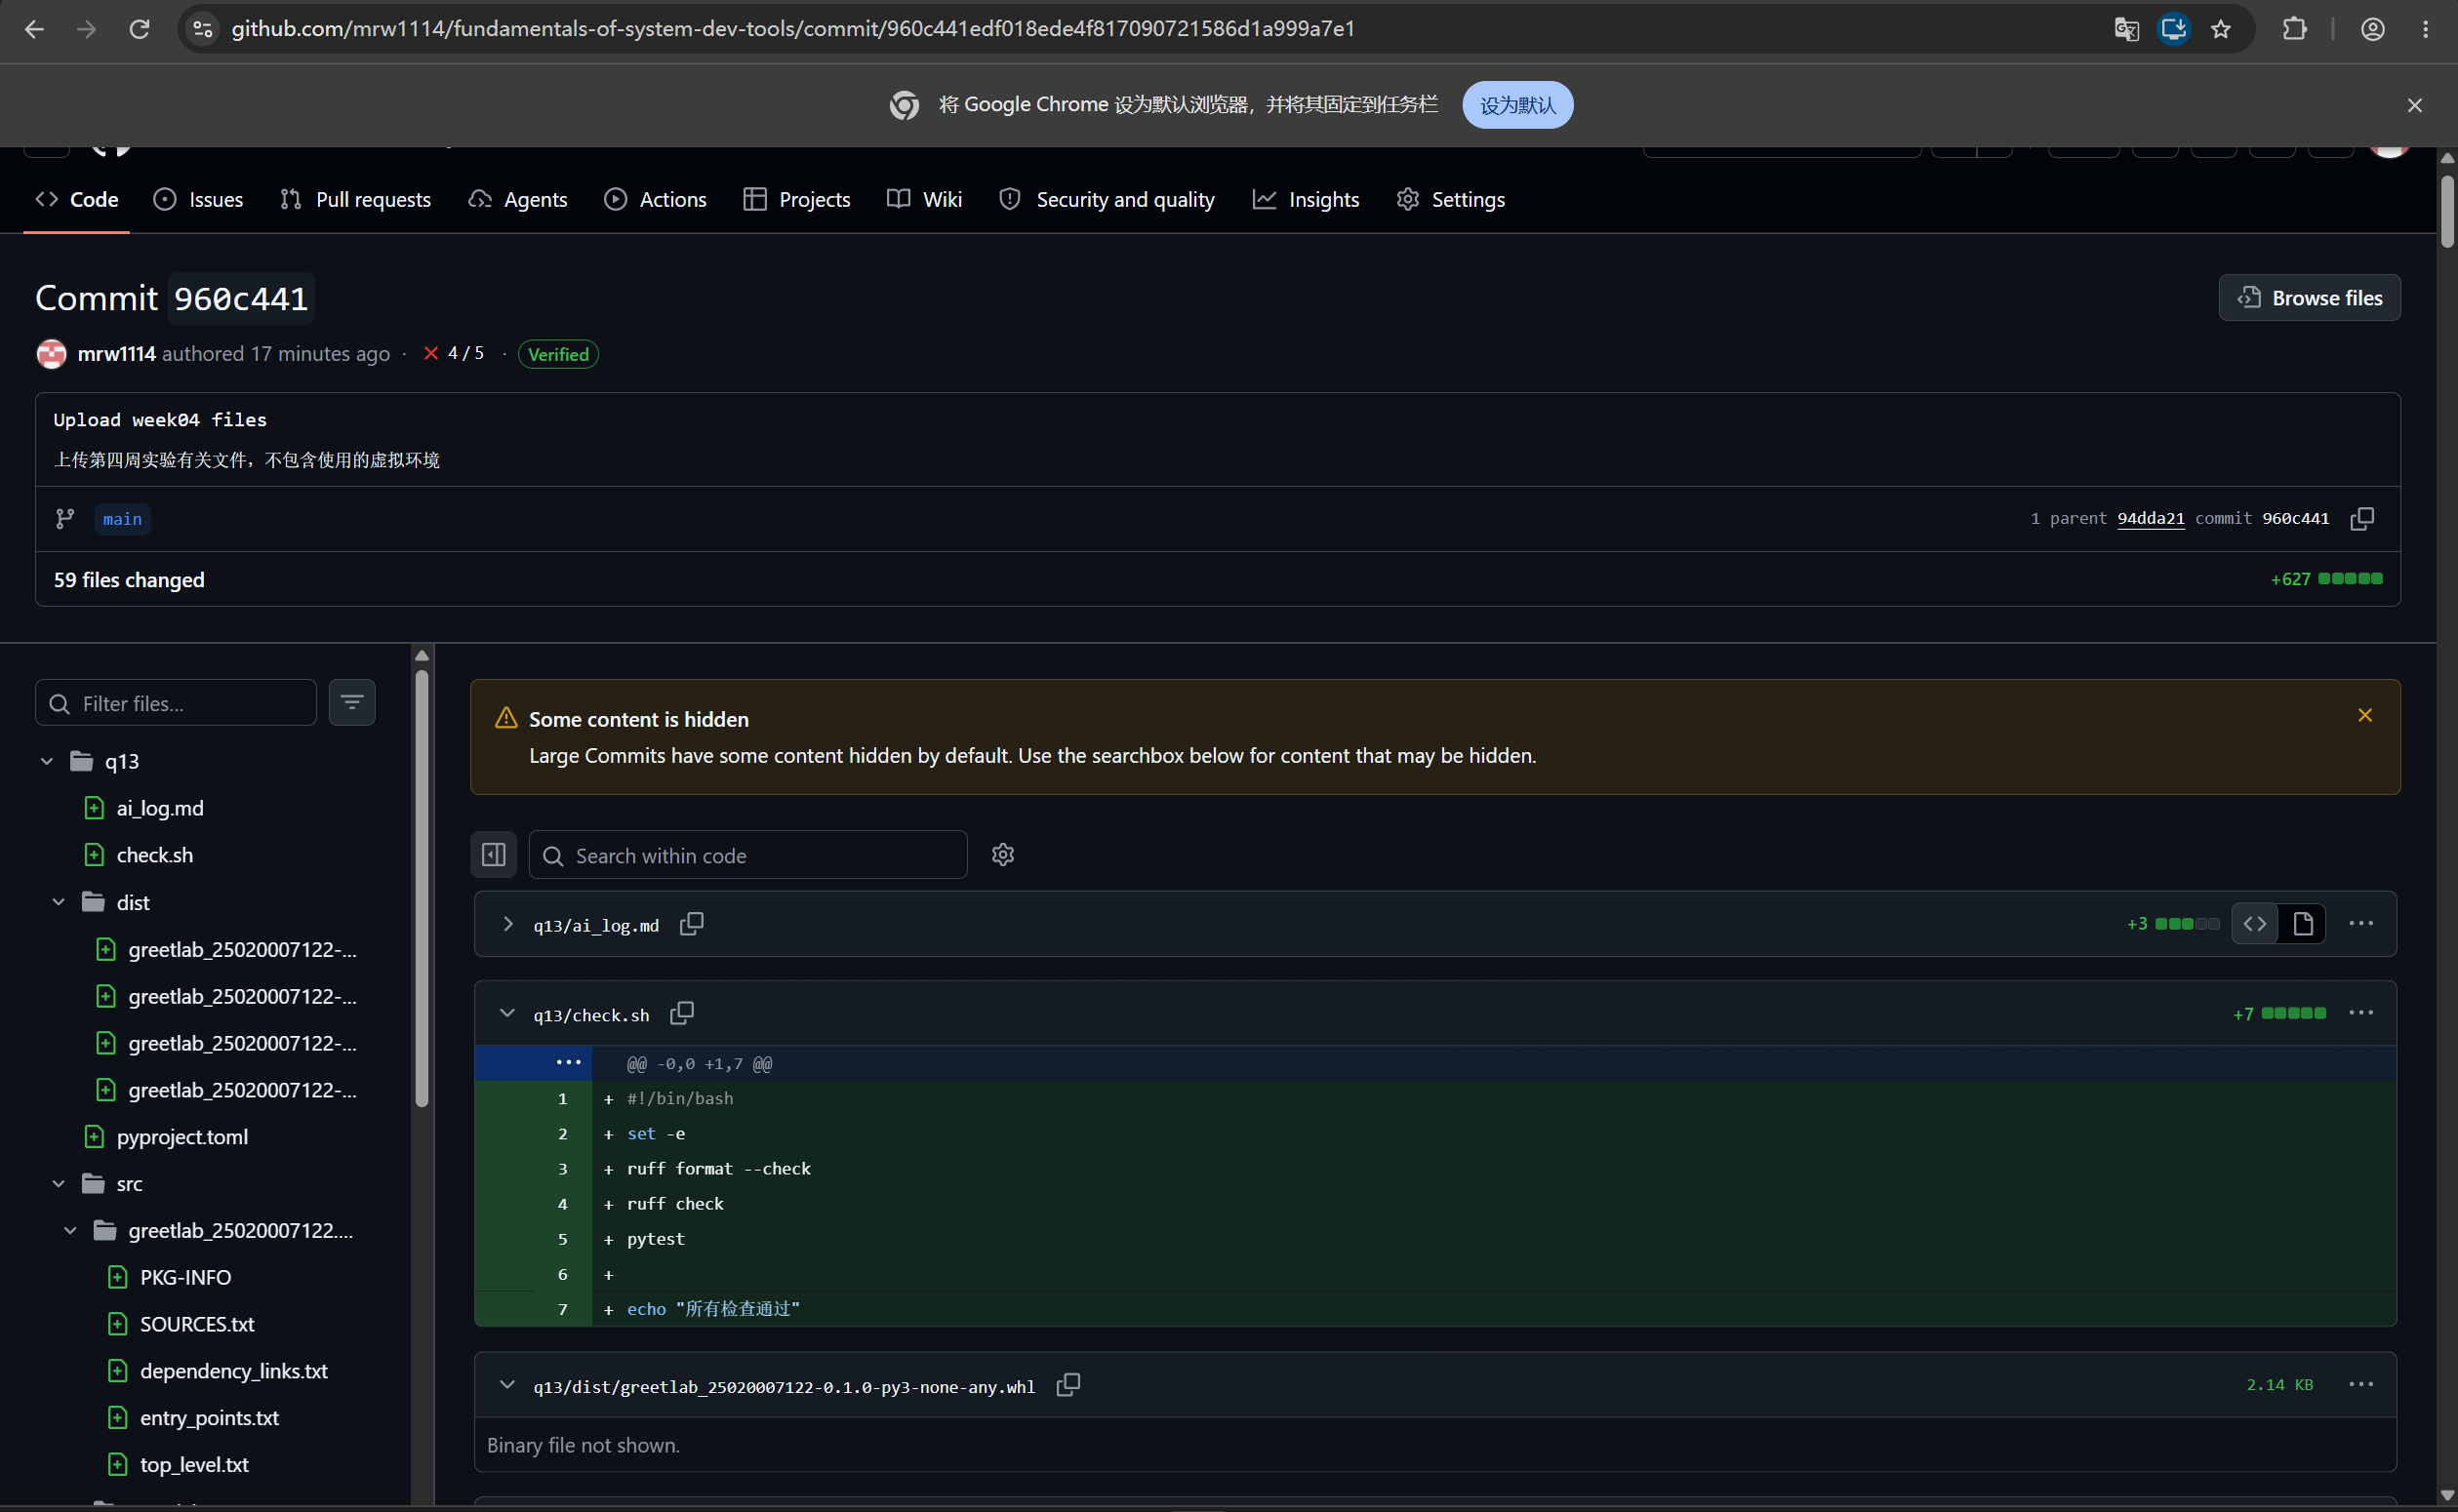
\includegraphics[width=\textwidth]{history4.png}
        \caption{commit 记录截图}
        \label{history4}
      \end{figure}
\end{document}
